\documentclass[a4paper, 10pt]{article}
\usepackage[utf8]{inputenc}
\usepackage{verbatim}
\usepackage{listings}
\usepackage{graphicx}
\usepackage{a4wide}
\usepackage{color}
\usepackage{amsmath}
\usepackage{amssymb}
\usepackage[dvips]{epsfig}
\usepackage[toc,page]{appendix}
\usepackage[T1]{fontenc}
\usepackage{cite} % [2,3,4] --> [2--4]
\usepackage{shadow}
\usepackage{hyperref}
\usepackage{titling}
\usepackage{marvosym }
\usepackage{physics}

\usepackage{subcaption}
\usepackage[noabbrev]{cleveref}
\usepackage{wasysym}
\usepackage{changepage}


\renewcommand{\topfraction}{.85}
\renewcommand{\bottomfraction}{.7}
\renewcommand{\textfraction}{.15}
\renewcommand{\floatpagefraction}{.66}
\renewcommand{\dbltopfraction}{.66}
\renewcommand{\dblfloatpagefraction}{.66}
\setcounter{topnumber}{9}
\setcounter{bottomnumber}{9}
\setcounter{totalnumber}{20}
\setcounter{dbltopnumber}{9}


\setlength{\droptitle}{-10em}   % This is your set screw

\setcounter{tocdepth}{2}

\lstset{language=c++}
\lstset{alsolanguage=[90]Fortran}
\lstset{basicstyle=\small}
\lstset{backgroundcolor=\color{white}}
\lstset{frame=single}
\lstset{stringstyle=\ttfamily}
\lstset{keywordstyle=\color{red}\bfseries}
\lstset{commentstyle=\itshape\color{blue}}
\lstset{showspaces=false}
\lstset{showstringspaces=false}
\lstset{showtabs=false}
\lstset{breaklines}
\title{FYS4411 - Project 1\\
	Variational Monte Carlo}
\author{Daniel Heinesen, Gunnar Lange \& Aram Salihi}
\begin{document}
	\maketitle
	\begin{abstract}
	We present an investigation into hard-sphere bosons trapped in a harmonic-oscillator like trap, using the same set-up as \cite{DuBois2001}. This system is investigated using a variational Monte Carlo approach, with both the Metropolis and the Metropolis-Hastings algorithm. This is done both with and without an interaction potential between the bosons, and the results are compared to the analytic results and results found by a previous study (\cite{Kristiansen2016}), with the error being estimated using blocking. We are able to excellently reproduce the analytic results in the noninteracting case. In the interacting case, in an elliptical harmonic oscillator potential, we find an excellent agreement for 10 particles (0.23\% deviation) but a somewhat poorer agreement for 50 and 100 particles (1.52\% and 2.72\% deviation respectively).
	Finally, we also plot the onebody density for 10 particles both with and without interaction, and find that it qualitatively fits our picture of the system. The onebody density in the noninteracting case also reproduces the exact answer to within $0.5\%$. All scripts and some of the data used for this project are available at our \href{https://github.com/dulte/FYS4411/}{GIT repository.}\footnote{\url{https://github.com/dulte/FYS4411/}}
	\end{abstract}
	\newpage
	\tableofcontents
	\newpage
	\section{Introduction}
	Confined quantum mechanical systems have received considerable attention in the literature, as they have many possible novel applications, ranging from qubits to energy storage. The existence of Bose-Einstein condensation in gases of certain alkali atoms, has sparked the interest in confined bosonic systems in particular (see e.g. \cite{Nilsen2005}). \\
	\linebreak
	We present an investigation into a system of hard-sphere bosons trapped in a harmonic oscillator well, based on the work by \cite{DuBois2001}. We model our bosons as spheres with radius $a$, and investigate systems both with and without a repulsive interaction preventing them from moving through one another. We then use a variational Monte Carlo (VMC) simulation to estimate the ground-state energy of our system.\\
	\linebreak
	 We seek to understand how the ground-state energy of the system depends on various parameters such as the number of particles in the system, the shape of the trap and the way we sample in our variational Monte Carlo method. We compare our results with analytic results or previous studies wherever they are available. We also investigate methods for quickly determining an approximation to the optimal variational parameter, using a gradient descent method, to avoid performing more than a few large VMC calculations. Finally, we look at the onebody density of our system, to get a feel for how the bosons are distributed throughout our system.
	\section{Theoretical model}
	We investigate bosons in a potential trap. The Hamiltonian of such a system for $N$ bosons is in general given by:
	\begin{equation} \label{eq:general_Hamiltonian}
	H=\sum_{i=1}^N\left(-\frac{\hbar^2}{2m}\nabla_i^2 +V_{ext}(\boldsymbol{r}_i)\right)+\sum_{i<j}^N V_{int}(\boldsymbol{r}_i, \boldsymbol{r}_j)
	\end{equation}
	Where $V_{ext}$ is the external potential, i.e. the potential of the trap, whereas $V_{int}$ is the interal potential, i.e. the interaction potential between the bosons. We wish to approximate the ground state energy of our system described by the Hamiltonian given in equation \ref{eq:general_Hamiltonian}.
	\subsection{The potentials employed}
	\subsubsection{The external potential}
	We will focus on two different trap shapes: spherical and elliptical. The spherical trap can be described by a standard harmonic oscillator potential, which is given by:
	\begin{equation}
	V_{ext}(\boldsymbol{r})=\frac{1}{2}m\omega^2 r^2 \quad \mathrm{(spherical\  trap)}
	\end{equation}
	Where $m$ is the mass of the bosons and $\omega$ is a parameter characterizing the strength of the potential (the characteristic frequency of the trap). The elliptical trap, however, is given by:
	\begin{equation}
	V_{ext}(\boldsymbol{r})=\frac{1}{2}m[\omega^2 (x^2+y^2)+\omega_z^2 z^2] \quad \mathrm{(elliptical\  trap)}
	\end{equation}
	I.e. we allow the strength of the potential to be anisotropic in one direction, which we designate as the $z$-axis.
	\subsubsection{The internal potential}
	We will begin by investigating models where there is no repulsion between the bosons, however, we later add a repulsive potential that prevents bosons from occupying the same point in space. We define our internal potential as:
	\begin{equation}
	V_{int}(a,|\boldsymbol{r}_i-\boldsymbol{r}_j|)= 
	\begin{cases}
	\infty & \quad |\boldsymbol{r}_i-\boldsymbol{r}_j| \leq  a\\
	0 & \quad |\boldsymbol{r}_i-\boldsymbol{r}_j|>  a\\
	\end{cases}
	\end{equation}
	Where $a$ is a typical diameter of our bosons (the hard-core diameter), which equals the scattering length of the single boson potential.
	This potential thus represents the impossibility of bosons to occupy the same point in space.
	\subsection{The variational method}
	\subsubsection{The variational principle}
	To find the ground state energy, $E_0$ of bosons trapped in a potential, we employ the variational method. The variational principle states (according to \cite{Griffiths2004}) that:
	\begin{equation}\label{eq:Variational_principle}
	E_0\leq  \frac{\langle \Psi_T |H|\Psi_T \rangle}{\langle \Psi|\Psi\rangle}
	\end{equation}
	Where $H$ is the Hamiltonian of our system and $\Psi_T$ is \textit{any} trial wavefunction. We therefore choose a functional class for $\Psi_T$, which includes a free parameter. By varying this parameter, we can find an upper bound for the ground state energy. If our chosen functional form is reasonably close to the exact wavefunction, $\Psi$ of the system, then our estimate for $E_0$ should be reasonably close to the actual ground state energy of our system.
	\subsubsection{Choosing a trial wavefunction}
	As noted above, we should choose our trial wavefunction to be reasonably close to the expected form of the actual position wavefunctions of our system. We note first that the external potential represents a harmonic oscillator. For the harmonic oscillator, it is well known from introductory quantum mechanics that the eigenfunctions are Gaussians for each particle separately. Note that the elliptic oscillator has a preferred direction (the $z$-axis). We accommodate for this by introducing a parameter $\beta$, representing the asymmetry of the elliptical oscillator. We therefore choose our trial wavefunction for this part of the potential to be:
	\begin{equation}
	h(\boldsymbol{r}_1, ..., \boldsymbol{r}_N, \alpha, \beta)=\prod_{i=1}^N g(\alpha,\beta, \boldsymbol{r}_i)=\prod_{i=1}^N \exp[-\alpha(x_i^2+y_i^2+\beta z_i^2)]=\exp[-\alpha \sum_{i=1}^N (x_i^2+y_i^2+\beta z_i^2)]
	\end{equation}
	Where we now have two variational parameters, $\alpha$ and $\beta$. Here $\beta$ tunes the strength of the potential as a whole, whereas $\beta$ tunes the asymmetry of the spherical oscillator. We fix $\beta$ to be either $1$ (spherical trap) or $\beta=2.82843$ (elliptic trap) as specified by \cite{Nilsen2005}, and vary only $\alpha$.\\
	\linebreak
	For the internal potential, we expect a function that attenuates our wavefunction down to zero if the distance between any pair of particles becomes less than $a$. We choose this function to be continuous, on physical grounds. A simple choice for such a function is:
	\begin{equation}
	f(a,|\boldsymbol{r}_i-\boldsymbol{r}_j|)= 
	\begin{cases}
	0 & \quad |\boldsymbol{r}_i-\boldsymbol{r}_j| \leq  a\\
	1-\frac{a}{|\boldsymbol{r}_i-\boldsymbol{r}_j|} & \quad |\boldsymbol{r}_i-\boldsymbol{r}_j|>  a\\
	\end{cases}
	\end{equation}
	Where $\boldsymbol{r_i}$ represents the position of particle $i$. Putting this together, gives our trial wavefunction as:
	\begin{equation}\label{eq:trial_wavefunction}
	\Psi_T(\boldsymbol{r}_1, \boldsymbol{r}_2, ..., \boldsymbol{r}_N, \alpha, \beta)=\prod_ig(\alpha,\beta, \boldsymbol{r}_i)\prod_{i<j}f(a, |\boldsymbol{r}_i-\boldsymbol{r}_j|)
	\end{equation}
	This is thus the wavefunction that we will be using in equation \ref{eq:Variational_principle} to find our upper bound on the ground state energy. Note that the wavefunction does not need to be normalized to be employed in equation \ref{eq:Variational_principle}. We therefore disregard normalization of the trial wavefunction.
	\subsection{Analytic results in the simplest case}
	For $\beta=1$ (spherical trap) and $a=0$ (no interaction amongst the particles), our system reduces to a simple harmonic oscillator, for which analytic results are available. For a single particle, the ground-state energy is (according to \cite{Griffiths2004}) given by:
	\begin{equation}
	E=\frac{\hbar \omega d}{2}
	\end{equation}
	Where $d$ is the number of dimensions. For $N$ non-interacting particles this turns into:
	\begin{equation}\label{eq:Exact_Energy_N_particles}
	E=\frac{N\hbar \omega d}{2}
	\end{equation}
	The exact ground-state wavefunction for the harmonic oscillator is (in atomic units, as will be introduced in section \ref{sec:UNITS}) given by:
	\begin{equation}
	\exp\left(-\frac{\sum_{i=1}^d x_i^2}{2}\right)
	\end{equation}
	For $N$ non-interacting particles this turns into:
	\begin{equation}
	\prod_{i=1}^N 	\exp\left(-\frac{\sum_{i=1}^d x_i^2}{2}\right)
	\end{equation}
	Comparing this with our trial wavefunction in equation \ref{eq:trial_wavefunction}, shows that we should expect the ground-state energy to be achieved for:
	\begin{equation}\label{eq:exact_alpha}
	\alpha=0.5
	\end{equation}
	\subsection{Variational Monte Carlo methods}
	Note that equation \ref{eq:Variational_principle} involves two integrals over $3N$ dimensions. This is usually not possible to evaluate analytically for large $N$, and traditional numerical methods such as gaussian quadrature are far too slow in high dimensions to be feasible. We therefore employ variational Monte Carlo methods to help in evaluating these integrals. To do this, we consider these integrals to represents stochastic quantities, and define the probability distribution as:
	\begin{equation}
	P(\boldsymbol{r}_1, \boldsymbol{r}_2,...,\boldsymbol{r}_N, \alpha,\beta)=\frac{|\Psi_T|^2}{\int d\boldsymbol{r}_1d\boldsymbol{r}_2...d\boldsymbol{r_n}|\Psi_T|^2}
	\end{equation}
	Now define a new quantity, the local energy, as:
	\begin{equation}\label{eq:Local_energy_general_expression}
	E_L(\boldsymbol{r}_1, \boldsymbol{r}_2,...,\boldsymbol{r}_N, \alpha,\beta)=\frac{1}{\Psi_T}H\Psi_T
	\end{equation}
	The	expectation value of the Hamiltonian (i.e. the estimate of the energy) now turns into:
	\begin{equation}\label{eq:Expectation_Hamiltonian}
	E[H(\alpha, \beta)]=\int P(\boldsymbol{r}_1, \boldsymbol{r}_2,...,\boldsymbol{r}_N, \alpha,\beta)E_L(\boldsymbol{r}_1, \boldsymbol{r}_2,...,\boldsymbol{r}_N, \alpha,\beta)d\boldsymbol{r}_1d\boldsymbol{r}_2...d\boldsymbol{r}_N\approx \frac{1}{M}\sum_{i=1}^M E_{L,i}
	\end{equation}
	Where now $M$ is the number of Monte Carlo cycles, whereas $E_{L,i}$ is the local energy computed in the i-th Monte Carlo step. Note that the quality of this approximation is contingent upon our ability to sample our space. We employ two different algorithms for sampling our coordinate space.
	\subsubsection{The Metropolis algorithm}
	To move from one Monte Carlo step to the other, we will employ the Metropolis algorithm, as described in \cite{Hjorth-Jensen2015}. The algorithm works by sampling the probability distribution, but adding a bias to sample mostly in the regions where the probability distribution actually is large, to avoid wasting CPU cycles. The algorithm works by proposing a step:
	\begin{equation}
	\boldsymbol{r}_{p, new}=\boldsymbol{r}_p+\boldsymbol{\xi}dx
	\end{equation}
	Where $\boldsymbol{\xi}$ is a $d$-dimensional (with $d$ as the number of dimensions) vector of random numbers in $[0,1]$ and $dx$ is a chosen step size, which we tune as described in section \ref{sec:finding_optimal_step_size}. We then compute the ratio:
	\begin{equation}
	w=\frac{P(\boldsymbol{r}_1, ..., \boldsymbol{r}_{p,new}, ..., \boldsymbol{r}_n)}{P(\boldsymbol{r}_1, ..., \boldsymbol{r}_{p}, ..., \boldsymbol{r}_n)}=\frac{|\Psi_T(\boldsymbol{r}_1, ..., \boldsymbol{r}_{p,new}, ..., \boldsymbol{r}_n)|^2}{|\Psi_T(\boldsymbol{r}_1, ..., \boldsymbol{r}_{p}, ..., \boldsymbol{r}_n)|^2}
	\end{equation}
	This ratio determines whether the new position has a higher or lower value of the PDF than the old position. We then accept the move if and only if $w\geq \theta$, where $\theta\in [0,1]$ is a uniformly distributed random variable. This ensures that some steps that decrease the value of the PDF are accepted (giving a spread of value), but that we mostly sample where the PDF is large (which avoids wasting CPU cycles). It is possible to show (see e.g. \cite{Hjorth-Jensen2015}) that these wavefunctions do not need to be normalized. We therefore do not ever have to compute the normalization explicitly.
	\subsubsection{The Metropolis-Hastings algorithm (importance sampling)}\label{sec:Metropolis_Hasting_Sampling}
	The simple Metropolis algorithm described above assigns no preferred direction $\boldsymbol{dx}$ for the proposed step. This can be improved by adding a force term, "pushing" the Monte Carlo loop towards the region where the PDF is large. This is described in further detail in \cite{Hjorth-Jensen2015}, where it is shown that the expression fur such a quantum force is given, for particle $k$, by:
	\begin{equation}
	\boldsymbol{F}_k(\boldsymbol{r}_1, ..., \boldsymbol{r}_N)=2\frac{1}{\Psi_T}\nabla_k \Psi_T
	\end{equation}
	We compute explicitly the expression for $\boldsymbol{F}$, using the trial wavefunction in equation \ref{eq:trial_wavefunction}, in appendix \ref{ap:analytic_expression_for_the_local_energy_and_quantum_force}. This gives:
	\begin{equation}
	\boldsymbol{F}_k=	 -4\alpha\boldsymbol{Q}_{k} +
	2\sum_{j \neq k}\frac{\boldsymbol{r}_{k} - \boldsymbol{r}_{j}}{r_{kj}}u'(r_{kj})
	\end{equation}
	Where we have defined $\boldsymbol{Q}_{k} = \left(x_{k}\boldsymbol{\hat{i}} + y_{k}\boldsymbol{\hat{j}} + \beta z_{k}\boldsymbol{\hat{k}}\right)$.
	A more detailed analysis (given in \cite{Hjorth-Jensen2015}) shows that the correct way to incorporate such a term into the Metropolis algorithm is by adding a transition probability term given by the Green's functions:
	\begin{equation}\label{eq:Greens_Function}
	G(\boldsymbol{r}_1,...,\boldsymbol{r}_N,\boldsymbol{r'}_1,...,\boldsymbol{r'}_N)=\frac{1}{(4\pi D \Delta t)^{3/2}}\sum_{i=1}^N \exp \left(-\frac{(\boldsymbol{r}_i-\boldsymbol{r'}_i-D\Delta t\boldsymbol{F}_i(\boldsymbol{r}'_1,...,\boldsymbol{r}'_N))^2}{4D\Delta t}\right)
	\end{equation}
	Where $\boldsymbol{r}_i$ are the coordinates prior to the move and $\boldsymbol{r'}_i$ are the coordinates after the move, $D$ is a diffusion constant (equal to $1/2$) and $\Delta t$ is a step parameter that we tune. 
	The effect of this term is to modulate the acceptance probability, $w$. This term is now given by:
	\begin{equation}
	w(\boldsymbol{r}_1,...,\boldsymbol{r}_N,\boldsymbol{r'}_1,...,\boldsymbol{r'}_N)=\frac{G(\boldsymbol{r}_1,...,\boldsymbol{r}_N,\boldsymbol{r'}_1,...,\boldsymbol{r'}_N)|\Psi_T(\boldsymbol{r}_1,...,\boldsymbol{r}_N)|^2}{G(\boldsymbol{r'}_1,...,\boldsymbol{r'}_N,\boldsymbol{r}_1,...,\boldsymbol{r}_N)|\Psi_T(\boldsymbol{r'}_1,...,\boldsymbol{r'}_N)|^2}
	\end{equation}
	Which leads to the modified Metropolis algorithm, the Metropolis-Hastings algorithm, where a move is accepted if and only if $w\geq \theta$ where $\theta\in [0,1]$ again is a uniformly distributed random variable. This method is computationally far more expensive than the brute-force Metropolis algorithm, but it leads to a  significantly larger number of accepted steps. For this method to be effective, we must also choose our proposed new step slightly different, as described further in section \ref{sec:finding_optimal_step_size}.
	\subsection{The local energy}
	Note that in  order to estimate the expectation value of the Hamiltonian we must, according to equation \ref{eq:Expectation_Hamiltonian} compute the local energy, given by equation \ref{eq:Local_energy_general_expression}, in every Monte Carlo step. The local energy can be rewritten as:
	\begin{equation}
	E_L=\frac{1}{\Psi_T}H\Psi_T =\sum_{i=1}^N\left(-\frac{\hbar^2}{2m\Psi_T}\nabla_i^2 \Psi_T+V_{\mathrm{ext}}(\boldsymbol{r}_i)\right)+\sum_{i<j}^N V_{\mathrm{int}}
	\end{equation}
	We compute this numerically, but we also include an analytic computation, using our trial wavefunction $\Psi_T$ defined in equation \ref{eq:trial_wavefunction}. This is done in detail in appendix \ref{ap:analytic_expression_for_the_local_energy_and_quantum_force}, and gives:
	\begin{align}\label{eq:Local_energy_all}
	\begin{split}
	E_{L} = -\frac{\hbar^{2}}{2m}\sum_{k}\left[
	4\alpha^{2}\boldsymbol{Q}_{k}^{2} - 4\alpha\boldsymbol{Q}_{k} + \sum_{j \neq k}\left(\frac{\boldsymbol{r}_{k} - \boldsymbol{r}_{j}}{r_{kj}}u'(r_{kj})\right)\right.
	\\ \left. + \sum_{i,j \neq k}\left(\frac{\boldsymbol{r}\cdot\boldsymbol{r} + \boldsymbol{r}_{j}\cdot\boldsymbol{r}_{i} - \boldsymbol{r}_{j}\cdot\boldsymbol{r}_{k} -\boldsymbol{r}_{k}\cdot\boldsymbol{r}_{i}}{r_{ki}r_{kj}}u'(r_{ki})u'(r_{kj})\right)\right.
	\\
	\left. + \sum_{j \neq k}\left(u''(r_{kj} + \frac{2}{r_{kj}}u'(r_{kj}))\right)\right]
	+ \sum_{k}V_{ext}(\boldsymbol{r}_{k}) + \sum_{i < j}V_{int}(\boldsymbol{r}_{i}, \boldsymbol{r}_{j})
	\end{split}
	\end{align}
	\subsection{Gradient descent method to find the optimal parameter $\boldsymbol{\alpha}$}\label{sec:Gradient_descent_theory}
	To reduce our search space, we use a minimization method to find an approximation to the optimal variational parameter, $\alpha$. This minimization method is run with relatively few Monte Carlo steps, and once an approximate optimal parameter is found, we perform the analysis with more Monte Carlo steps (100 times as many). As our parameter space is one-dimensional ($\alpha$ is the only variational parameter), we choose to implement a simple gradient descent algorithm. This is implemented as follows:
	\begin{equation}
	\alpha_{n+1}=\alpha_n-\gamma_n \frac{\partial E_L}{\partial \alpha} (\alpha_n)
	\end{equation}
	We choose an initial $\alpha_0$ close to the correct $\alpha$ from the non-interacting case, and then iteratively follow wherever the gradient is lower. We use an adaptive step-size, which decreases as the difference between points get closer (i.e. as we get closer to the minimum). We follow \cite{doi:10.1093/imanum/8.1.141} for this, using:
	\begin{equation}
	\gamma_n=\frac{(\alpha_n-\alpha_{n-1})+\epsilon}{[\frac{\partial E_L}{\partial \alpha}(\alpha_n)-\frac{\partial E_L}{\partial \alpha}(\alpha_{n-1})]}
	\end{equation}
	Where we, however, implement add an additional parameter $\epsilon$ (compared to \cite{doi:10.1093/imanum/8.1.141}) to ensure that we do not get stuck at the same $\alpha$ values. Furthermore, we also implement an additional test that checks if $\frac{\partial E_L}{\partial \alpha}(\alpha_n)-\frac{\partial E_L}{\partial \alpha}(\alpha_{n-1})$ is less than a treshold, in which case we reset $\gamma$ to the initial guess $\gamma_0$.\\
	\linebreak	
	To implement this, we require the derivative of the local energy with respect to the variational parameter. We show in appendix \ref{ap:derivative_of_local_energy} that this derivative is given by:
	\begin{equation}
	\frac{\partial E_L}{\partial \alpha}(\alpha_n)=2\left(\big\langle \frac{1}{\Psi_T}\frac{\partial \Psi_T}{\partial \alpha}E_L[\alpha_n]\big\rangle-\big\langle \frac{1}{\Psi_T}\frac{\partial \Psi_T}{\partial \alpha}\big\rangle \big\langle E_L[\alpha_n]\big\rangle\right)
	\end{equation}
	Where we note that both the local energy and the wavefunction depend on $\alpha$.
	\subsection{One-body densities}
	We are interested in investigating the probability of finding a single particle at a distance $r$ from the origin of our system. This is an important quantity, as it can be measured experimentally. We approach this through the concept of the one-body density. The one-body density is defined by:
	\begin{equation}\label{eq:OneBodyDensity}
	\rho(\boldsymbol{r_1})=\int d\boldsymbol{r_2}...d\boldsymbol{r_N}|\Psi_T(\boldsymbol{r_1},\boldsymbol{r_2},...,\boldsymbol{r_N})|^2
	\end{equation}
	Where $\boldsymbol{r_1}$ is the position of any particle. The integral is evaluated using Monte Carlo integration, as described in further detail in section \ref{sec:MetOneBody}.\\
	\linebreak
	We also compute the expected value of our density distribution for the noninteracting case in an isotropic trap. We show in section \ref{ap:Expectation_value_onebody} that this expectation value is:
	\begin{equation}\label{eq:expectation_value_onebody}
	\langle r \rangle =\frac{2}{\sqrt{\pi}}
	\end{equation}
	\section{Methods}\label{Method_section}
	\subsection{A note on units}\label{sec:UNITS}
	The scattering-length for a typical BEC condensate atom is somewhere in the range $85<a<140a_0$, where $a_0$ is the Bohr radius. The characteristic trap length (at 0 K), however, is $a_{ho}=(\hbar/m\omega)^{1/2}\approx 10^{4}$Å$-2\cdot 10^{4}$Å, as described in further detail in \cite{DuBois2001}. We introduce length units of $a_{ho}$ and energy units of $\hbar \omega$. We show in appendix \ref{ap:dimensionless_hamiltonian} that, using these units, the Hamiltonian can be rewritten as:
	\begin{equation}\label{eq:Hamiltonian_dimensionless}
	H=\sum_{i=1}^N\left(-\nabla_i^2 + x_i^2+y_i^2+\gamma^2 z_i^2\right)+\sum_{i<j}V_{int}(\boldsymbol{r}_i, \boldsymbol{r}_j)
	\end{equation}
	Where $\gamma=\omega_z/\omega$.
	\subsection{Implementing the interacting case}
	To implement the interacting case ($a\neq 0$), we follow the parameters used by \cite{Nilsen2005}. We therefore let $a=0.0043$ and $\omega_z=\beta=2.82843$ (with $\omega=1$). We find the optimal $\alpha$ in the interacting case by using the gradient descent method described in section \ref{sec:Gradient_descent_theory}, using $100$ times fewer Monte Carlo cycles in the gradient descent calculations than in the full simulation.
	\subsection{Outline of the structure of our program}
	Our program uses the \texttt{Eigen} library in \texttt{C++} to keep track of the matrices. We implement three main classes:\\
	\paragraph{\texttt{main.cpp}}
	This class reads in the parameters from an input file, sets up parallelization in MPI and starts a new simulation.\\
	\linebreak
	\paragraph{\texttt{simulation.cpp}}
	This class contains the gradient descent method, as well as a method that actually runs the main Monte Carlo loop. The onebody densities are also computed in this class.\\
	\linebreak
	\paragraph{system.ccp}
	This class distributes the particles in the system, sets up the grid, calculates the wavefunction, proposes new steps and checks the acceptance of the steps. 
	\subsection{Proposing a new position}
	To propose a new step, we use a different method for the brute force method versus the importance sampling method. For the brute force method, we propose a new step as:
	\begin{equation}
	\boldsymbol{r}^i_{\mathrm{new}}=\boldsymbol{r}^i_{\mathrm{old}}+\boldsymbol{\xi} dx
	\end{equation}
	Where $\boldsymbol{r}^i_{\mathrm{old}}$ is the previous position of particle $i$ and $\boldsymbol{\xi}$ is a normally distributed variable with mean $0$ and standard deviation $1$. We tune the parameter $dx$ for the brute force simulation, as described in section \ref{sec:finding_optimal_step_size} and \ref{sec:Disc_optimal_step_size_brute_force} and find that we get good results for $dx=0.5$.\\
	\linebreak
	For importance sampling, however, we propose a different step to keep the statistics consistent (as discussed in \cite{Hjorth-Jensen2015}). The new step is then given by:
	\begin{equation}
	\boldsymbol{r}^i_{\mathrm{new}}=\boldsymbol{r}^i_{\mathrm{old}}+\boldsymbol{\xi} \sqrt{dt}+D\boldsymbol{F}_idt
	\end{equation}
	Where $\boldsymbol{F_i}$ is the quantum force on particle $i$ and $D$ is the diffusion parameter, discussed in section \ref{sec:Metropolis_Hasting_Sampling}. The parameter $dt$ is the same parameter used in the Greens function (equation \ref{eq:Greens_Function}), and we find it by looking at the energy for the exactly solvable system for different $dt$, as described in section \ref{sec:finding_optimal_step_size}. We find that we get good results for $dt=0.05$, as discussed in section and \ref{sec:Disc_importance_sampling_step_size}.
	\subsection{Finding the optimal step size}\label{sec:finding_optimal_step_size}
	For the brute-force Monte Carlo sampling, we must estimate an optimal step size, $d x$, with which to move our step. For the Monte Carlo simulation with importance sampling, we must similarly estimate the parameter $dt$. These step sizes should ensure that:
	\begin{itemize}
		\item The simulation quickly converges to the correct energy
		\item The variance quickly stabilizes
	\end{itemize}
	To find these properties, we look at how the variance and the mean of the local energy (across every Monte Carlo sample) varies as we increase the number of Monte Carlo cycles. We investigate various values of $dx$ (respectively $dt$). For each of these values, we ensure that we manage to hit an energy minimum at $\alpha=0.5$ in the noninteracting case.\\
	\linebreak
	We measure the variance in the standard way (i.e. not using blocking), as blocking requires the number of steps to be a power of $2$. We do this for the noninteracting system, using $\alpha=0.45$ (as the exact $\alpha$ gives essentially $0$ variance). \\
	\linebreak
	We then choose the $dx$ (respectively $dt$) that ensure that the variance and the mean quickly stabilize.
	\subsection{Statistical treatment of the data}\label{sec:Blocking}
	We wish to estimate the statistical errors of the local energy. As subsequent values for the local energy are based on the previous values of the local energy, we are dealing with a correlated time series. The normality assumptions usually employed when generating confidence intervals therefore does not hold. Instead, we use blocking to estimate the error in our energy. A detailed mathematical treatment of this method is found in \cite{Jonsson2018}. We therefore present only the algorithm. Assume that we have $n$ observations $Q^0=\{Q_1^0,...,Q_n^0\}$ of the local energy, and we wish to estimate the variance of the local energy. The uncorrelated estimator for the standard deviation is given by:
	\begin{equation}
	s=\sqrt{\frac{1}{n-1}\sum_{i=1}^n (Q_i-\overline{Q})^2}
	\end{equation}
	Where $\overline{Q}$ is the mean of the local energy estimates. This expression is only valid in the uncorrelated case, however. The idea of blocking is to perform iterative transformations of the data, until the covariance of the data is approximately zero. Specifically, the transformation that we will be implementing is the following:
	\begin{equation}
	Q^i \rightarrow Q^{i+1}: Q^{i+1} = \left\{ \frac{Q^i_1+Q^i_2}{2}, \frac{Q^i_3+Q^i_4}{2},...,\frac{Q^i_{n-1}+Q^i_{n}}{2}\right\}
	\end{equation}
	We choose $n$ to be a power of $2$, i.e. $n=2^d$, as this enables us to perform this transformation a maximum of $d$ times. We now define an estimator for the covariance between observations that are distance $h$ apart by:
	\begin{equation}
	\hat{\gamma^k}(h)=\frac{1}{n}\sum_{i=1}^{n-h}(Q_i^k-\overline{Q}^k)(Q_{i+h}^k-\overline{Q}^k)
	\end{equation}
	We are interested in knowing when $\gamma^k(1)\approx 0$. This can be found by hand, simply by realizing that the transformation $Q^i \rightarrow Q^{i+1}$ described above preserves the variance of the data. It is shown in \cite{Jonsson2018} that $\gamma^k(1) \rightarrow 0$ for successive iterations, and therefore a plot of the empirical variance as a function of iterations should eventually stabilize, giving the variance. \\
	\linebreak
	We use an alternative, automatic, approach to estimate when the covariance is small. This is based on comparing our results to a $\chi^2$ distribution, and is described further in \cite{Jonsson2018}.
	\subsection{Implementing the onebody density}\label{sec:MetOneBody}
	To compute the one-body density defined by equation \ref{eq:OneBodyDensity}, we must compute the integral in that equation. We show in appendix \ref{ap:approximte_onebody_density} that, if we only consider the radial distribution of the onebody density, this integral can be discretized as:
	\begin{equation}
		\rho(r_i)\approx \frac{N_i}{4\pi r_i^2 \Delta r}
		\end{equation}
		Where $N_i$ is the number of particles in the spherical shell with radius $r_i$ to $r_i+\Delta r$. Thus, to compute the onebody density, we run our Monte Carlo simulation and check in which shell the particle that we move at every step is located. We also check numerically that the normalization is correct (i.e. that the area under the curve equals the total number of particles).
	\subsection{Parallelizing our code}
	We note that our algorithms are embarrassingly parallel, as they do not need to communicate between one another to span a large portion of the parameter space. We therefore run 4 cores simultaneously, producing 4 times as much data. This data is simply appended in the blocking method, giving $4$ times more data, and thus better estimates of the mean and the standard deviation.
	\newpage
	\section{Results}
	\subsection{Finding the optimal step size}
We plot the mean and the variance for various steps sizes, as discussed in section \ref{sec:finding_optimal_step_size}. This gives the plot shown in figure \ref{fig:find_dx_noimportance} for the brute force sampling. As discussed further in section \ref{sec:Disc_optimal_step_size_brute_force}, we choose $dx=0.5$ as our parameter for the brute-force case.\\
	\begin{figure}[ht!]
		\centering
			\centering
			\begin{subfigure}{.5\textwidth}
				\centering
				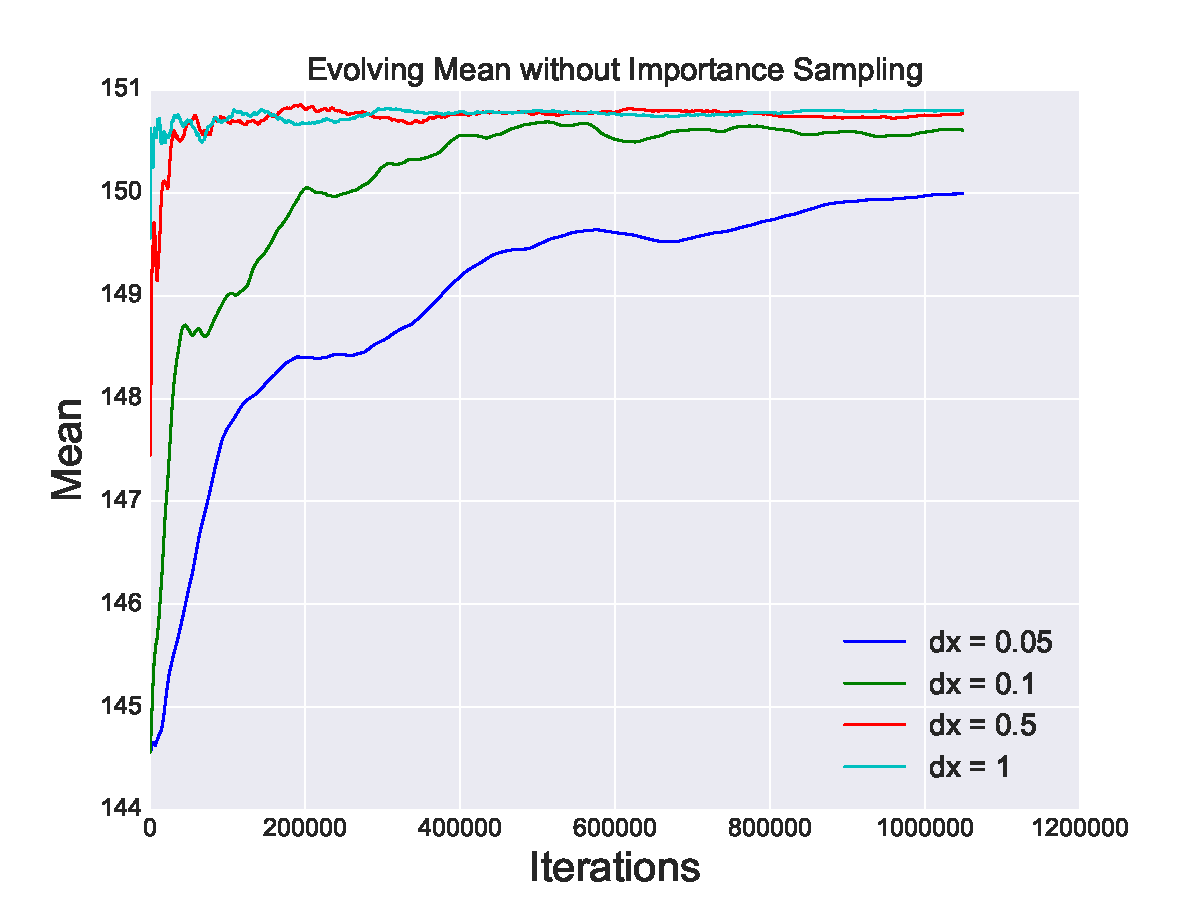
\includegraphics[width=.8\linewidth]{../Results/Finding_the_optimal_step_size/EvoMean.pdf}
				\caption{Mean energy}
			\end{subfigure}%
			\begin{subfigure}{.5\textwidth}
				\centering
				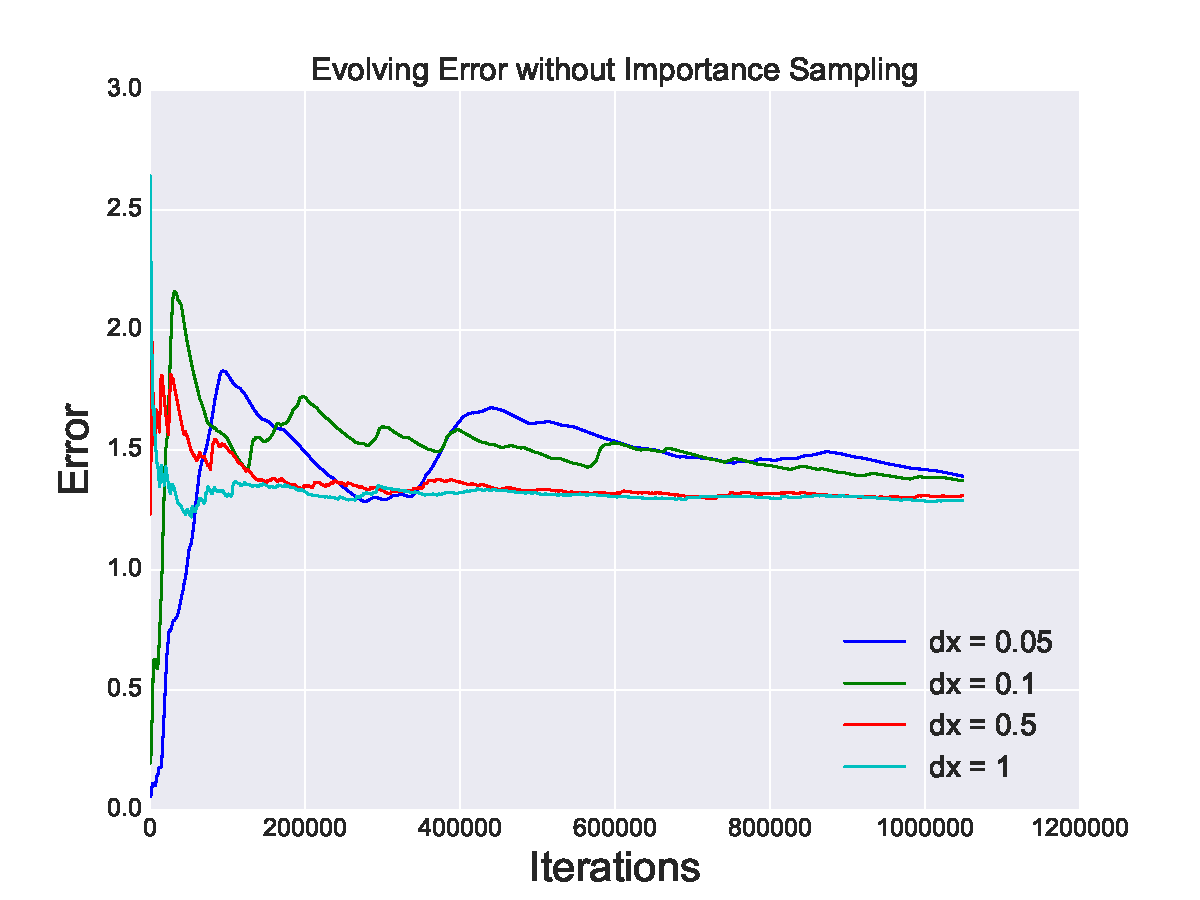
\includegraphics[width=.8\linewidth]{../Results/Finding_the_optimal_step_size/EvoStd.pdf}
				\caption{Standard deviation of the energy}
			\end{subfigure}
			\caption{Mean energy and standard deviation of the energy as a function of Monte Carlo cycles for various step sizes, $dx$. This was done without importance sampling in three dimensions, using $N=100$, $a=0$ (noninteracting), $\alpha=0.45$, $\omega_z=1$, $\beta=1$, $\omega=1$}\label{fig:find_dx_noimportance}
	\end{figure}
	\linebreak
 We produce a similar plot for the case with importance sampling. This gives the plots shown in figure \ref{fig:find_dx_importance}. As explained in section \ref{sec:Disc_importance_sampling_step_size}, we choose $dt=0.05$. \\
	\linebreak
		\begin{figure}[ht!]
			\centering
			\centering
			\begin{subfigure}{.5\textwidth}
				\centering
				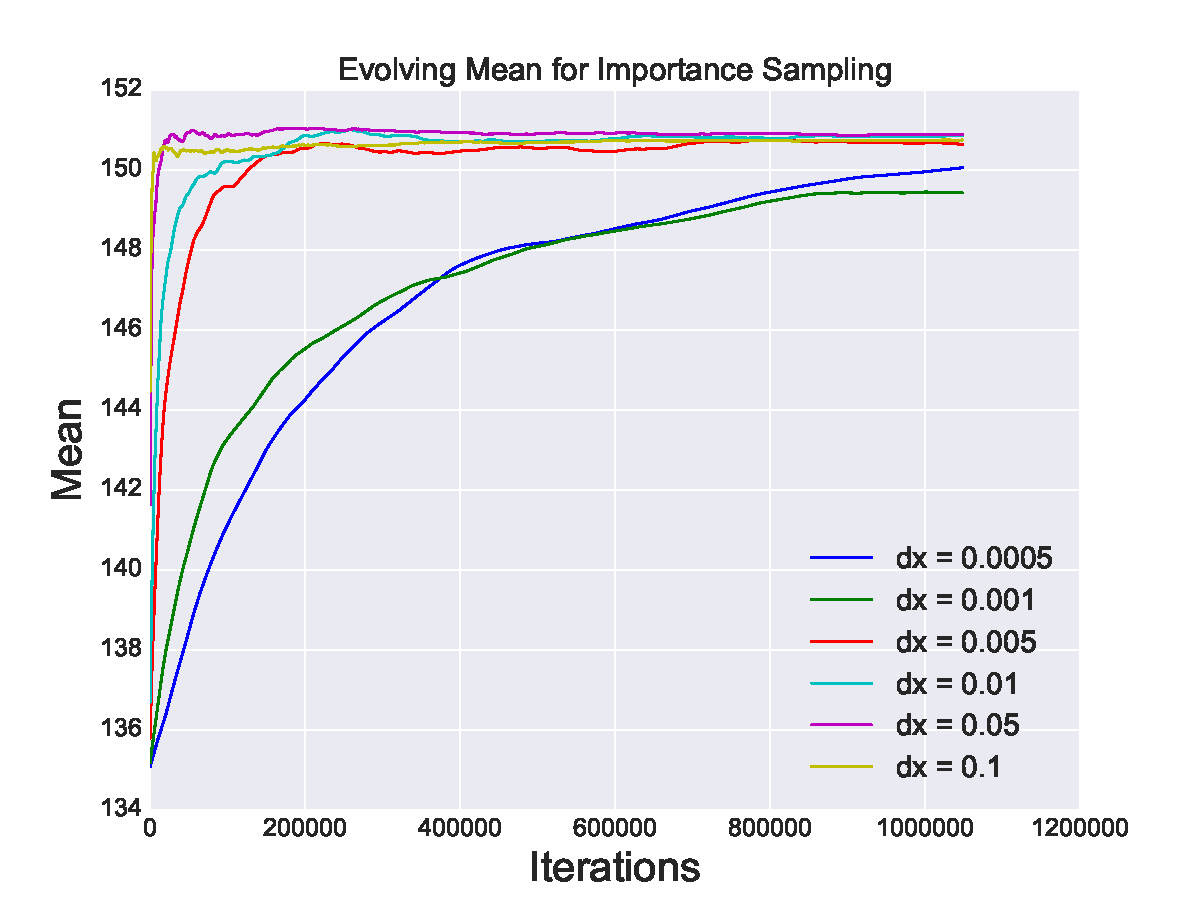
\includegraphics[width=.8\linewidth]{../Results/Finding_the_optimal_step_size/EvoMeanIS.pdf}
				\caption{Mean energy}
			\end{subfigure}%
			\begin{subfigure}{.5\textwidth}
				\centering
				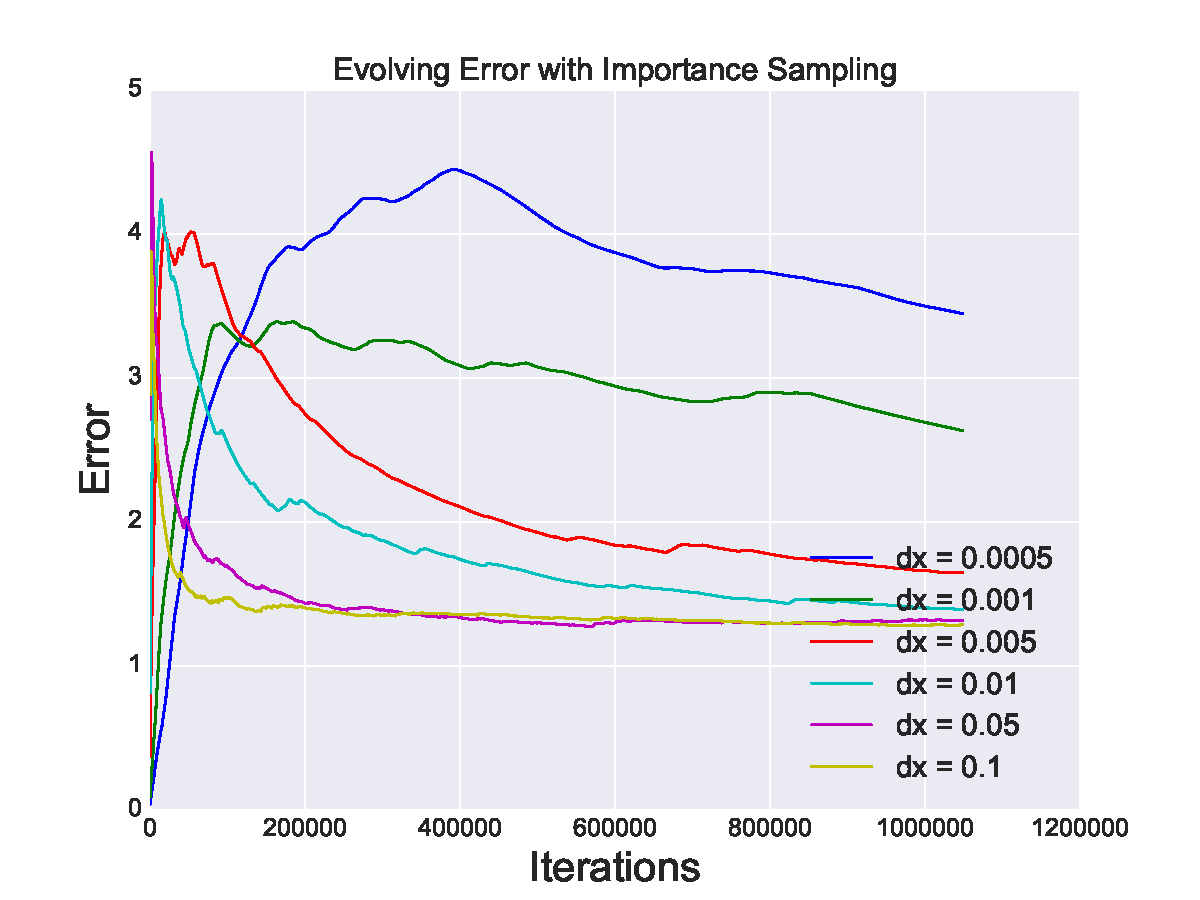
\includegraphics[width=.8\linewidth]{../Results/Finding_the_optimal_step_size/EvoStdIS.pdf}
				\caption{Standard deviation of the energy}
			\end{subfigure}
			\caption{Mean energy and standard deviation of the energy as a function of Monte Carlo cycles for various step sizes, $dx$. This was done with importance sampling in three dimensions, using $N=100$, $a=0$ (noninteracting), $\alpha=0.45$, $\omega_z=1$, $\beta=1$, $\omega=1$}\label{fig:find_dx_importance}
		\end{figure}
	\subsection{Testing our code}
	We test our code by running the simulations for the noninteracting case ($a=0$) and for the correct value of the variational parameter, $\alpha=0.5$. We then expect our code to reproduce the exact energy given in equation \ref{eq:Exact_Energy_N_particles}. We test this using both the analytic and the numeric energy, and time the CPU difference between them.  We compute the uncertainty using the blocking method, as described in section \ref{sec:Blocking}. We show the results without importance sampling in table \ref{tab:4.1_benchmark_no_Green} (1D), table \ref{tab:4.1_benchmark_no_Green_2D} (2D)  and table \ref{tab:4.1_benchmark_no_Green_3D} (3D).\\
	\begin{table}[ht!]
		\caption{Benchmarking of our code in the noninteracting case ($a=0$), in one dimension, showing the analytic energy (computed by means of equation \ref{eq:Local_energy_all}), the numeric energy and the exact energy (given by equation \ref{eq:Exact_Energy_N_particles}). This is for the spherical trap ($\omega=\omega_z=\beta=1$) in one dimension. This was obtained using $4$ cores, each running $2^{20}$ Monte Carlo cycles. The simulation with the numeric energy for $N=500$ took too long to be feasible. Wherever no uncertainty is specified, blocking gave an error of $0$. This is with brute force sampling.}\label{tab:4.1_benchmark_no_Green}
		\begin{adjustwidth}{-2cm}{}
			\begin{tabular}{cccccc}
				N & Analytic energy, $E_a$ [$\hbar \omega$] & Numeric energy, $E_n$ [$\hbar \omega$] & Exact energy, $E$ [$\hbar \omega$]& CPU time $E_a$ [s] &CPU time $E_n$ [s]\\
				\hline
				1&$0.5$&$0.5$&$0.5$& 1.41&2.03\\
				10&$5$&$5.00000\pm 1\cdot 10^{-5}$&$5$& $1.47$&9.13\\
				100&$50$&$50.001\pm 0.001$&$50$&2.42&446.83\\
				500&$250$&-&250 &51.02 &-
			\end{tabular}
		\end{adjustwidth}
	\end{table}
	\begin{table}[ht!]
		\caption{Same table as table \ref{tab:4.1_benchmark_no_Green}, but in 2 dimensions}\label{tab:4.1_benchmark_no_Green_2D}
		\begin{adjustwidth}{-2cm}{}
			\begin{tabular}{cccccc}
				N & Analytic energy, $E_a$ [$\hbar \omega$] & Numeric energy, $E_n$ [$\hbar \omega$] & Exact energy, $E$ [$\hbar \omega$]& CPU time $E_a$ [s] &CPU time $E_n$ [s]\\
				\hline
				1&$1$&$1$&$1$& 1.32&2.27\\
				10&$10$&$10.00000\pm 3\cdot 10^{-5}$&$10$& $1.49$&15.11\\
				100&$100$&$100.000\pm 0.003$&$50$&2.65&810.2\\
				500&$500$&- &$500$&49.2 &-
			\end{tabular}
		\end{adjustwidth}
	\end{table}
		\begin{table}[ht!]
			\caption{Same table as table \ref{tab:4.1_benchmark_no_Green}, but in 3 dimensions}\label{tab:4.1_benchmark_no_Green_3D}
			\begin{adjustwidth}{-2cm}{}
				\begin{tabular}{cccccc}
					N & Analytic energy, $E_a$ [$\hbar \omega$] & Numeric energy, $E_n$ [$\hbar \omega$] & Exact energy, $E$ [$\hbar \omega$]& CPU time $E_a$ [s] &CPU time $E_n$ [s]\\
					\hline
					1&$1.5$&$1.5$&$1.5$& 1.56&2.85\\
					10&$15$&$15.00000\pm 6\cdot 10^{-5}$&$15$& $1.91$&29.89\\
					100&$150$&$149.997\pm 0.005$&$150$&3.92&1791.83\\
					500&$750$&- &$750$&54.36 &-
				\end{tabular}
			\end{adjustwidth}
		\end{table}
		\linebreak
		We do a similar analysis with importance sampling. This gives table \ref{tab:4.1_benchmark_Green} (1D), table \ref{tab:4.1_benchmark_Green_2D} (2D) and table \ref{tab:4.1_benchmark_Green_3D} (3D). As discussed further in section \ref{sec:Disc_energy_as_a_function_of_alpha} , we opt to not use importance sampling in the interacting case.
		 \begin{table}[ht!]
		 	\caption{Benchmarking of our code in the noninteracting case ($a=0$), in one dimension, showing the analytic energy (computed by means of equation \ref{eq:Local_energy_all}), the numeric energy and the exact energy (given by equation \ref{eq:Exact_Energy_N_particles}). This is for the spherical trap ($\omega=\omega_z=\beta=1$) in one dimension. This was obtained using $4$ cores, each running $2^{20}$ Monte Carlo cycles. The simulation with the numeric energy for $N=500$ took too long to be feasible. Wherever no uncertainty is specified, blocking gave an error of $0$. This is with importance sampling.}\label{tab:4.1_benchmark_Green}
			\begin{adjustwidth}{-2cm}{}
				\begin{tabular}{cccccc}
					N & Analytic energy, $E_a$ [$\hbar \omega$] & Numeric energy, $E_n$ [$\hbar \omega$] & Exact energy, $E$ [$\hbar \omega$]& CPU time $E_a$ [s] &CPU time $E_n$ [s]\\
					\hline
					1&$0.5$&$0.5$&$0.5$& 1.83&2.36\\
					10&$5$&$4.99999\pm 2\cdot 10^{-5}$&$5$& $2.03$&9.59\\
					100&$50$&$49.997\pm 0.001$&$50$&4.92&441.62\\
					500&$250$&-&250 &56.83 &-
				\end{tabular}
			\end{adjustwidth}
		\end{table}
		 \begin{table}[ht!]
			 \caption{Same as table \ref{tab:4.1_benchmark_Green} but in 2 dimensions.}\label{tab:4.1_benchmark_Green_2D}
		 	\begin{adjustwidth}{-2cm}{}
		 		\begin{tabular}{cccccc}
		 			N & Analytic energy, $E_a$ [$\hbar \omega$] & Numeric energy, $E_n$ [$\hbar \omega$] & Exact energy, $E$ [$\hbar \omega$]& CPU time $E_a$ [s] &CPU time $E_n$ [s]\\
		 			\hline
		 			1&$1$&$1$&$1$& 1.87&2.80\\
		 			10&$10$&$10.00004\pm 3\cdot 10^{-5}$&$10$& $2.16$&16.86\\
		 			100&$100$&$99.998\pm 0.003$&$100$&5.71&808.74\\
		 			500&$500$&-&500 &58.17 &-
		 		\end{tabular}
		 	\end{adjustwidth}
		 \end{table}
		 \begin{table}[ht!]
		 	\caption{Same as table \ref{tab:4.1_benchmark_Green} but in 3 dimensions.}\label{tab:4.1_benchmark_Green_3D}
		 	\begin{adjustwidth}{-2cm}{}
		 		\begin{tabular}{cccccc}
		 			N & Analytic energy, $E_a$ [$\hbar \omega$] & Numeric energy, $E_n$ [$\hbar \omega$] & Exact energy, $E$ [$\hbar \omega$]& CPU time $E_a$ [s] &CPU time $E_n$ [s]\\
		 			\hline
		 			1&$1.5$&$1.5$&$1.5$& 1.87&3.08\\
		 			10&$15$&$14.99999\pm 6\cdot 10^{-5}$&$15$& $2.66$&26.26\\
		 			100&$150$&$149.997\pm 0.006$&$150$&6.40&1672.32\\
		 			500&$750$&-&750 &58.55 &-
		 		\end{tabular}
		 	\end{adjustwidth}
		 \end{table}
		 \pagebreak
	\subsection{Energy as a function of $\boldsymbol{\alpha}$}
	To investigate how our solution varies with $\alpha$, we plot the local energy as a function of the variational parameter $\alpha$. We first do this for the spherical harmonic oscillator ($\omega=\omega_z=\beta=1$) with no interaction ($a=0$), with $N=100$ and $2^{20}$ Monte Carlo cycles per core (running with $4$ cores). We also compute the error in each case, using the blocking method. This gives the plot shown in figure \ref{fig:Average_EL_N=100_brute_force} (brute-force sampling) and figure \ref{fig:Average_EL_N=100_importance} (importance sampling).\\
	\pagebreak	
		\begin{figure}[ht!]
			\centering
				\begin{subfigure}{1\textwidth}
					\centering
					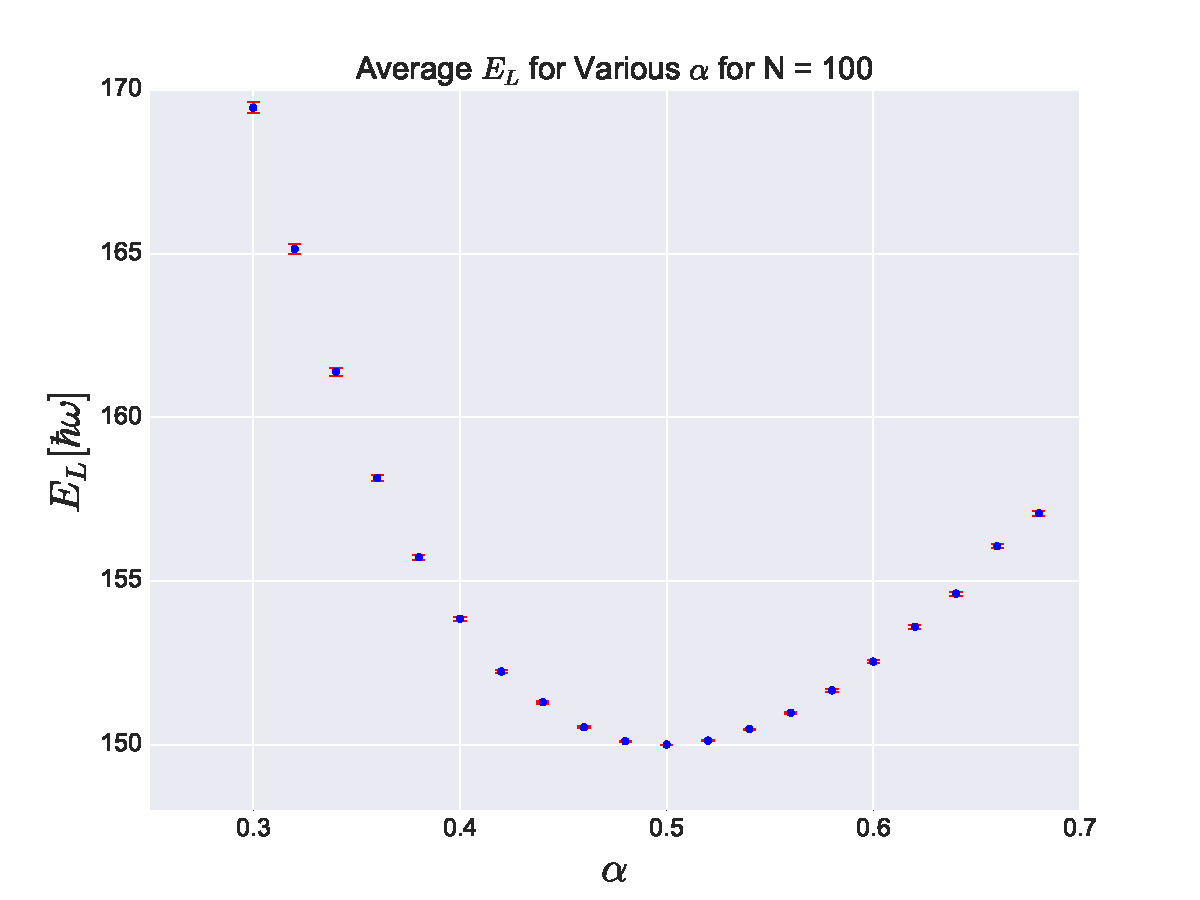
\includegraphics[width=.8\linewidth]{../Results/Energy_as_a_function_of_alpha/EvAlphaN100.pdf}
					\caption{Brute-force sampling}\label{fig:Average_EL_N=100_brute_force}
				\end{subfigure}
				\begin{subfigure}{1\textwidth}
					\centering
					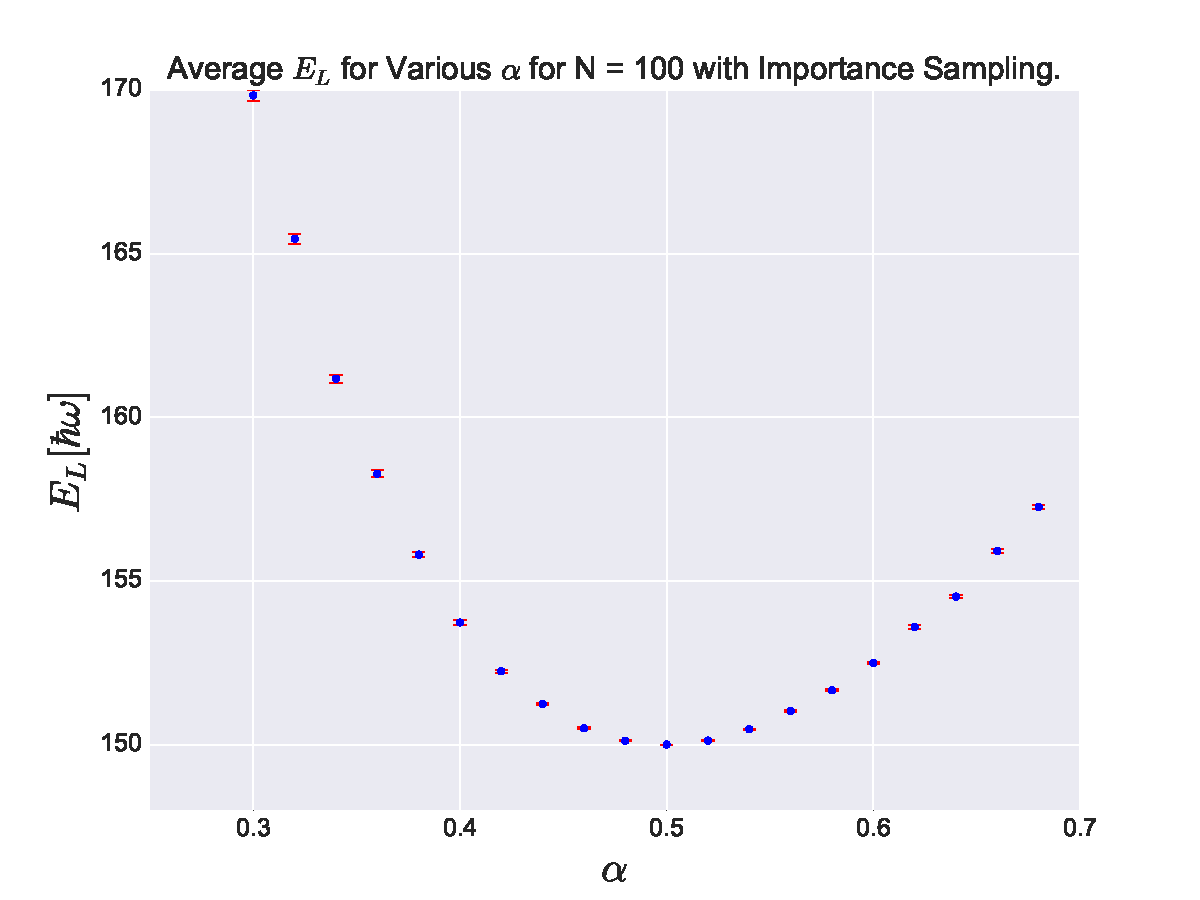
\includegraphics[width=.8\linewidth]{../Results/Energy_as_a_function_of_alpha/EvAlphaN100IS.pdf}
					\caption{Importance sampling}\label{fig:Average_EL_N=100_importance}
				\end{subfigure}
			\caption{Local energy for various values of $\alpha$, for $a=0$, $\beta=1$, $\omega=\omega_z=1$, $N=100$ in 3 dimensions using $2^{20}$ Monte Carlo cycles per core. This is done with both brute force and importance sampling.}
		\end{figure}
	\linebreak
	We do a similar analysis for $N=10$ in the interacting case\footnote{Any higher $N$ was far too slow.}. This gives the plot shown in figure \ref{fig:EL_alpha_N10_interacting} for brute-force sampling.
			\begin{figure}[ht!]
				\centering
				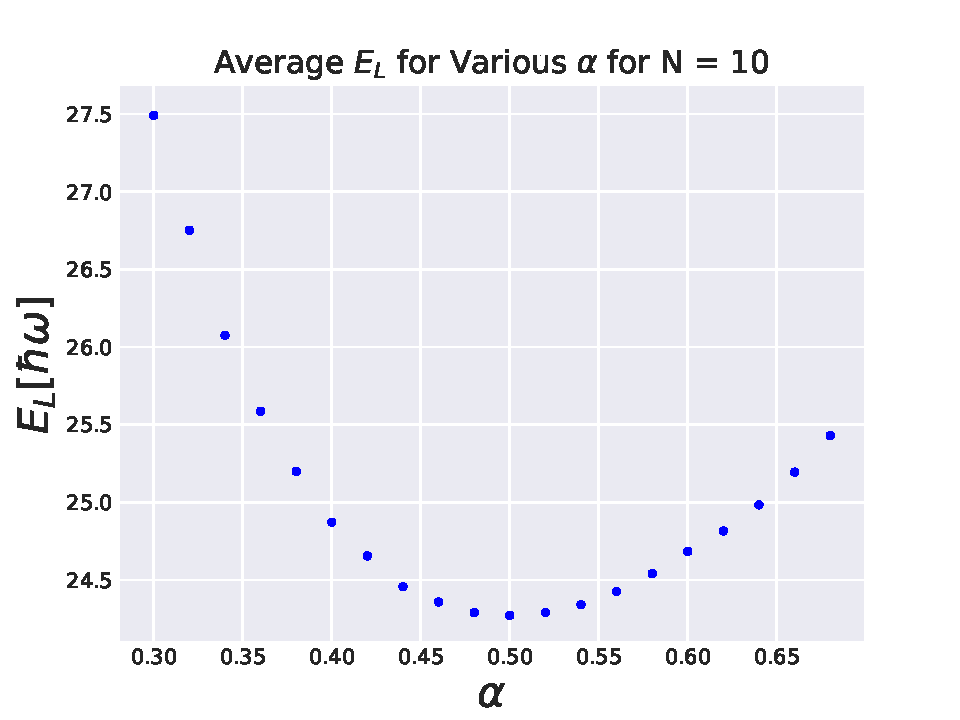
\includegraphics[scale=0.8]{../Results/Energy_as_a_function_of_alpha/Alpha_v_EL_Interacting_N10.pdf}
				\caption{Local energy for various values of $\alpha$, for $a=0.0043$, $\omega=1$, $\omega_z=\beta=2.82843$, $N=10$, 3 dimensions, $2^{20}$ Monte Carlo cycles per core, with 4 cores, and brute force sampling. The error bars are too small to be visible.}\label{fig:EL_alpha_N10_interacting}
			\end{figure}
	\subsection{Finding the optimal $\boldsymbol{\alpha}$}
	We run our gradient descent method for various $N$ in the fully interacting case, to find the optimal parameter. We first test our method by running it for the 3D noninteracting system of $10$ particles, and ensuring that it finds the correct value at $\alpha=0.5$. The result of this is shown in figure \ref{fig:gradient_descent_noninteracting}. 	The method finds $\alpha=0.5$ in few time steps. We do a similar analysis for the interacting case with $N=10,50$ and $100$. This is shown in figure \ref{fig:gradient_descent_interactingN10} (N=10), figure \ref{fig:gradient_descent_interactingN50} (N=50) and figure \ref{fig:gradient_descent_interactingN100} (N=100).
	\pagebreak
			\begin{figure}[ht!]
				\centering
				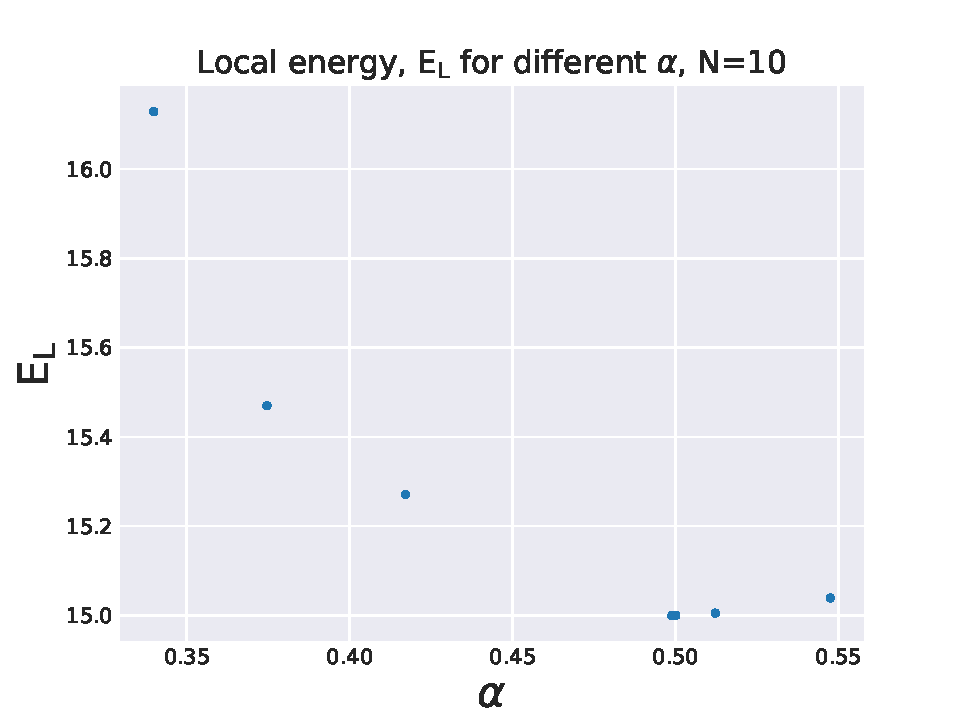
\includegraphics[scale=0.8]{../Results/Finding_the_optimal_alpha/E_v_alpha_gradient_noninteracting.pdf}
				\caption{Gradient descent for finding the optimal $\alpha$ in the noninteracting case ($a=0$), with $N=10$, $\omega=\omega_z=\beta=1$, 3 dimensions and brute-force sampling. We use a minimum step size, $\epsilon=10^{-6}$, and an accept whenever the gradient is less than $10^{-6}$.}\label{fig:gradient_descent_noninteracting}
			\end{figure}
		\begin{figure}[ht!]
			\centering
			\begin{subfigure}{.5\textwidth}
				\centering
				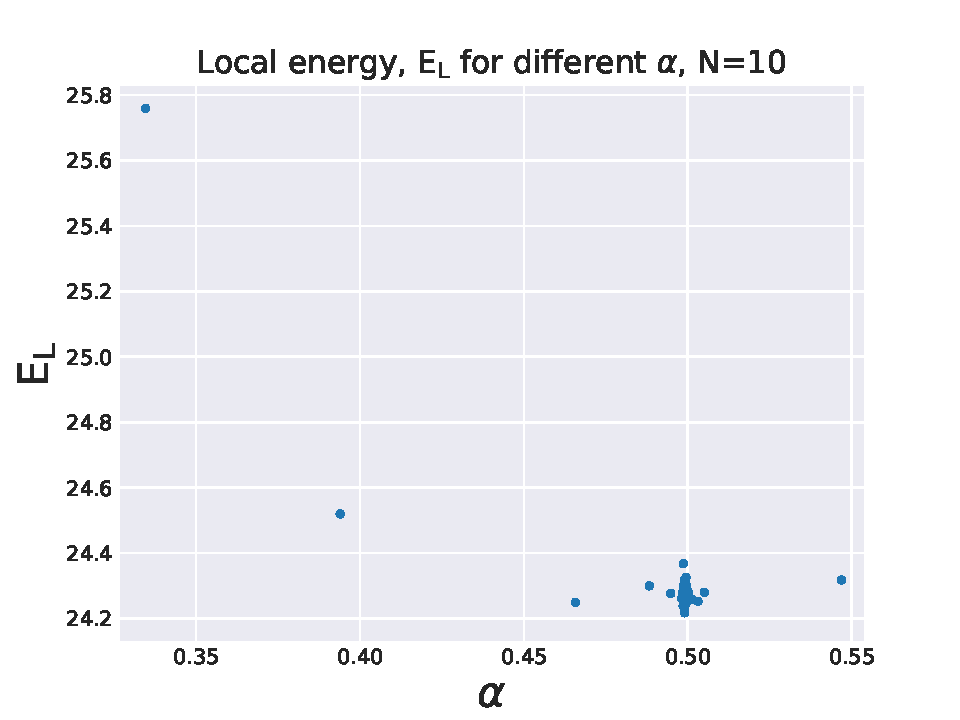
\includegraphics[width=.8\linewidth]{../Results/Finding_the_optimal_alpha/E_v_alpha_gradient.pdf}
				\caption{Gradient descent}
			\end{subfigure}%
			\begin{subfigure}{.5\textwidth}
				\centering
				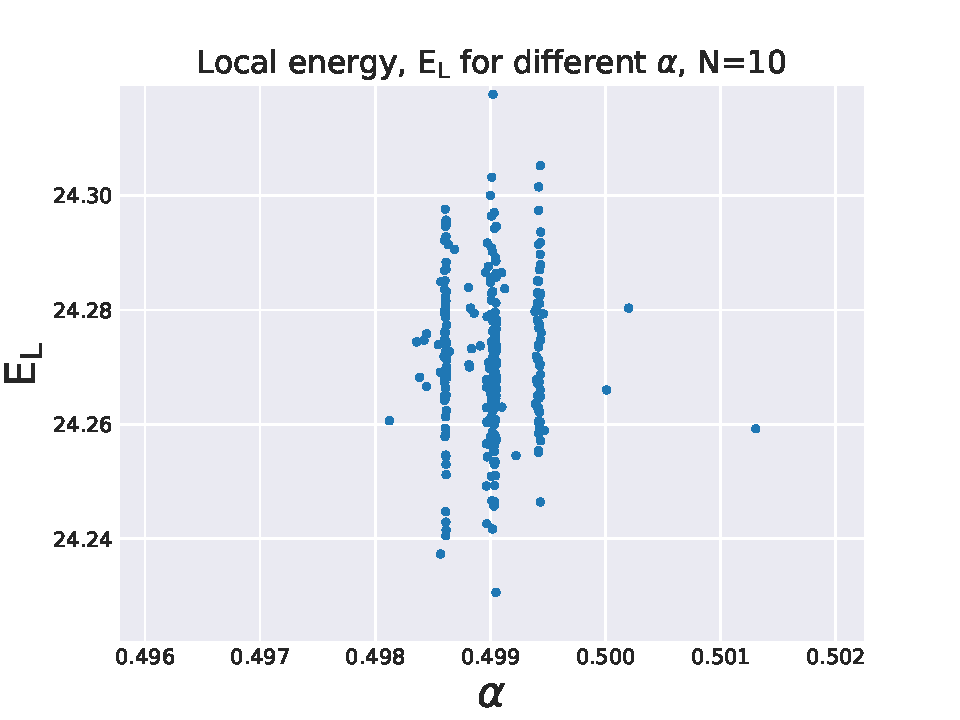
\includegraphics[width=.8\linewidth]{../Results/Finding_the_optimal_alpha/E_v_alpha_gradient_zoom.pdf}
				\caption{Zoomed in version}
			\end{subfigure}
			\caption{Gradient descent for finding the optimal $\alpha$ in the interacting case ($a=0.0043$), with $N=10$, $\omega=1$, $\omega_z=\beta=2.82843$, 3 dimensions and brute-force sampling. We use a minimum step size, $\epsilon=10^{-6}$, and an accept whenever the gradient is less than $10^{-6}$. We show also a zoomed-in version of the same plot.}\label{fig:gradient_descent_interactingN10}
		\end{figure}
				\begin{figure}[ht!]
					\centering
					\centering
					\begin{subfigure}{.5\textwidth}
						\centering
						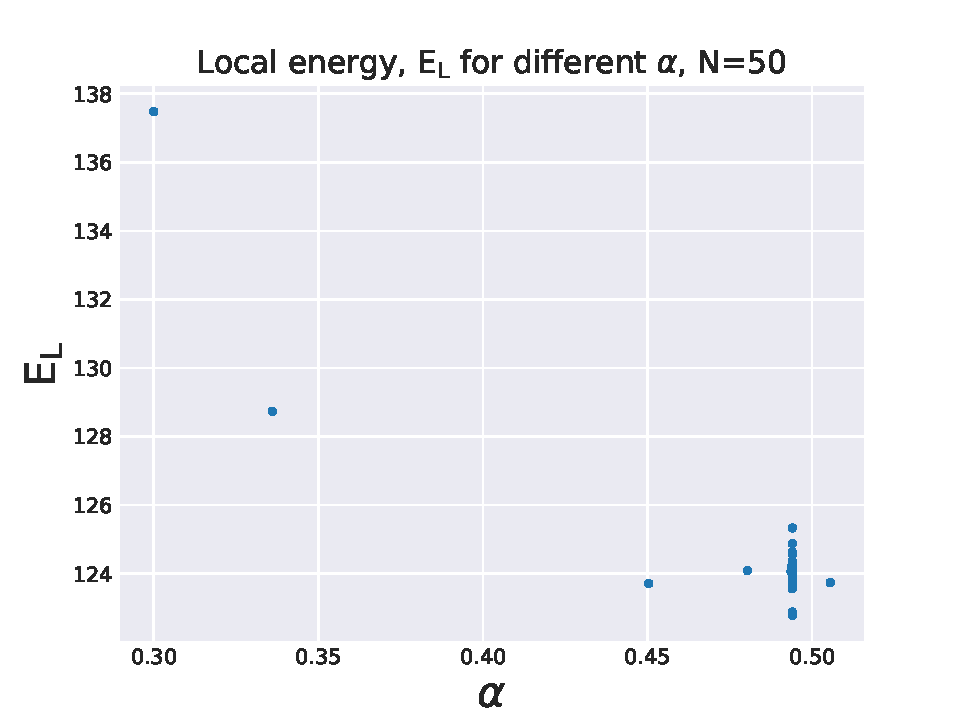
\includegraphics[width=.8\linewidth]{../Results/Finding_the_optimal_alpha/E_v_alpha_gradientN50.pdf}
						\caption{Gradient descent}
					\end{subfigure}%
					\begin{subfigure}{.5\textwidth}
						\centering
						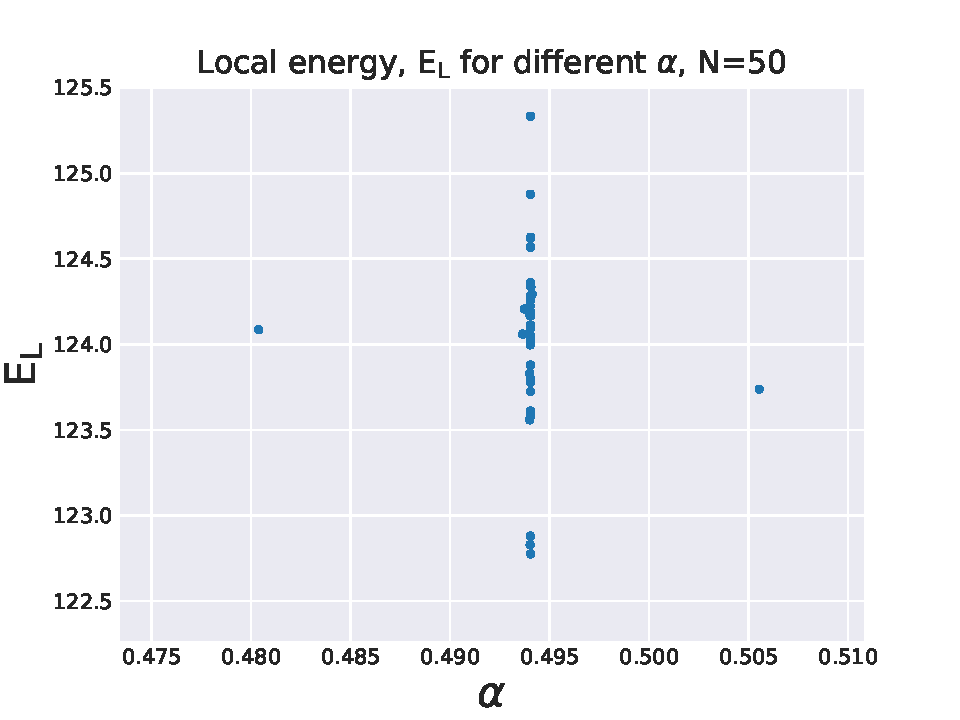
\includegraphics[width=.8\linewidth]{../Results/Finding_the_optimal_alpha/E_v_alpha_gradientN50Zoom.pdf}
						\caption{Zoomed in version}
					\end{subfigure}
					\caption{Same as figure \ref{fig:gradient_descent_interactingN10} but with $N=50$. }\label{fig:gradient_descent_interactingN50}
				\end{figure}
		\begin{figure}[ht!]
			\centering
			\centering
			\begin{subfigure}{.5\textwidth}
				\centering
				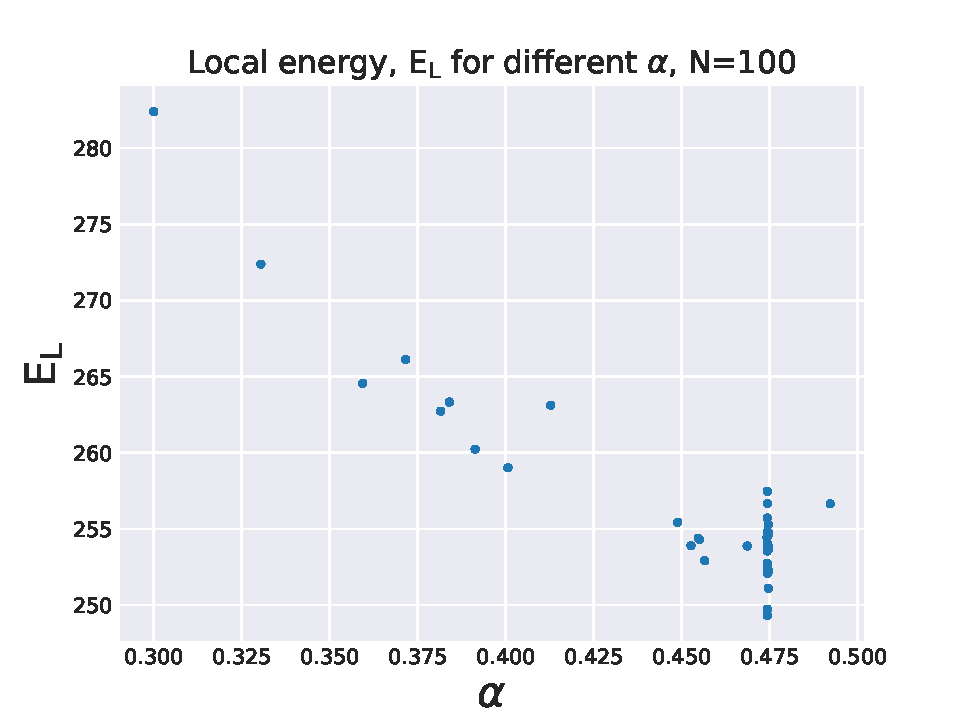
\includegraphics[width=.8\linewidth]{../Results/Finding_the_optimal_alpha/E_v_alpha_gradientN100.pdf}
				\caption{Gradient descent}
			\end{subfigure}%
			\begin{subfigure}{.5\textwidth}
				\centering
				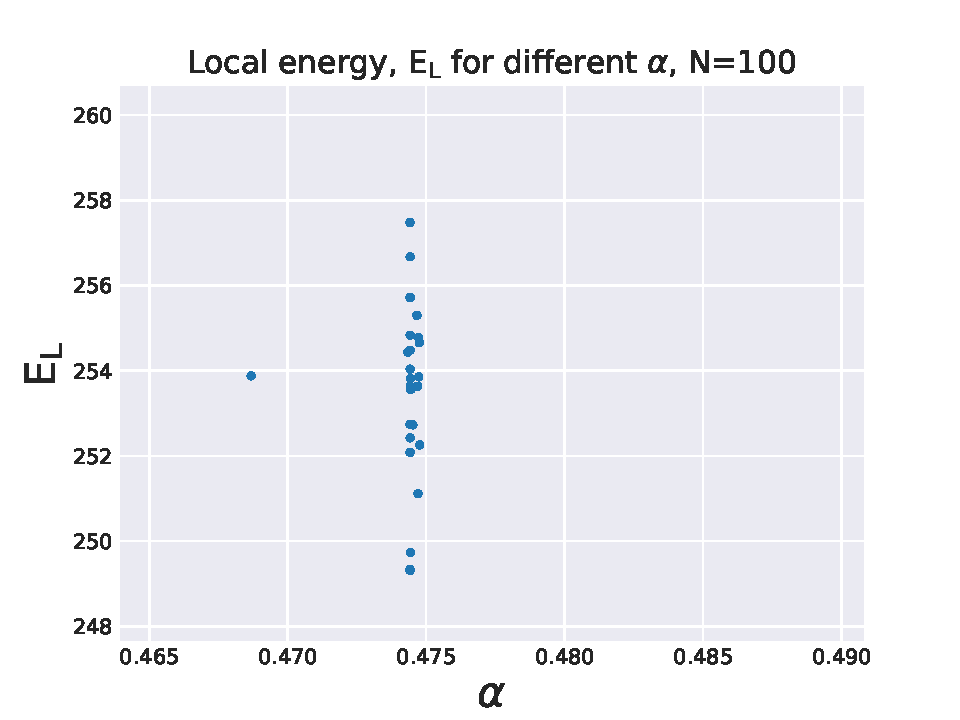
\includegraphics[width=.8\linewidth]{../Results/Finding_the_optimal_alpha/E_v_alpha_gradientN100Zoom.pdf}
				\caption{Zoomed in version}
			\end{subfigure}
			\caption{Same as figure \ref{fig:gradient_descent_interactingN10} but with $N=100$. }\label{fig:gradient_descent_interactingN100}
		\end{figure}
		\pagebreak
		\newpage
		We summarize the values found by our optimization method in table \ref{tab:correct_alpha_interacting}.
			\begin{table}[ht!]
			\caption{Values for the variational parameter $\alpha$ for various $N$. This was estimated in 3 dimensions, with $a=0.0043$, $\omega=1$, $\omega_z=\beta=2.82843$ and using brute force sampling with $2^{20}/100$ timesteps. We stopped the gradient descent method once either the gradient was less than $10^{-6}$, or after a maximum of $40$ iterations was reached.}\label{tab:correct_alpha_interacting}
				\centering
				\begin{tabular}{cccc}
					N & $\alpha$\\
					\hline
					10 & $0.499037$\\
					50 &$0.494033$\\ 
					100 & $0.474419$
				\end{tabular}
		\end{table}
	\subsection{Results from the fully interacting system}
	We now run the fully interacting system. We choose the parameters used by \cite{Nilsen2005}, and an $\alpha$ value found by the gradient descent as shown in table \ref{tab:correct_alpha_interacting}. We do not use importance sampling, as it took too long. We use the analytic expression for the local energy, given in equation \ref{eq:Local_energy_all}, and  compare our results to the study quoted in \cite{Kristiansen2016}. This gives the values shown in table \ref{tab:fully_interacting_system}.
	\begin{table}[ht!]
		\caption{Local energy in 3 dimensions for the fully interacting system. We use the parameters used by \cite{Nilsen2005}, i.e. $a=0.0043$, $\omega_z=\beta=2.82843$, $\omega=1$. We use brute force sampling, and the parameters $\alpha$ found by our gradient descent method, shown in table \ref{tab:correct_alpha_interacting}. This was estimated using $2^{20}$ Monte Carlo cycle per core, running on $4$ cores. The reference data are from \cite{Kristiansen2016}.}\label{tab:fully_interacting_system}
		\centering
		\begin{tabular}{ccccc}
			N & Local energy, $E_L$ [$\hbar \omega$] &Reference local energy, $E_{L,Ref}\ [\hbar \omega]$&Difference [\%]& CPU time [s]\\
			\hline
			10 & $24.14259\pm 9\cdot 10^{-5}$ &24.2&0.23& 78.4679\\
			50 & $123.859\pm 0.001$ &122& 1.52&4338.12\\
			100 & $253.7\pm 0.1$&247&2.72 &31734.3\\
			%100 & $253.12 \pm 0.06$ & 31442.4\\
		\end{tabular}
	\end{table}
	\pagebreak
	\subsection{Onebody densities}
	We plot the onebody density for the interacting and noninteracting case in figure \ref{fig:results_onebody} below. We find that the mean of this distribution is at $r=1.123$.
		\begin{figure}[ht!]
			\centering
			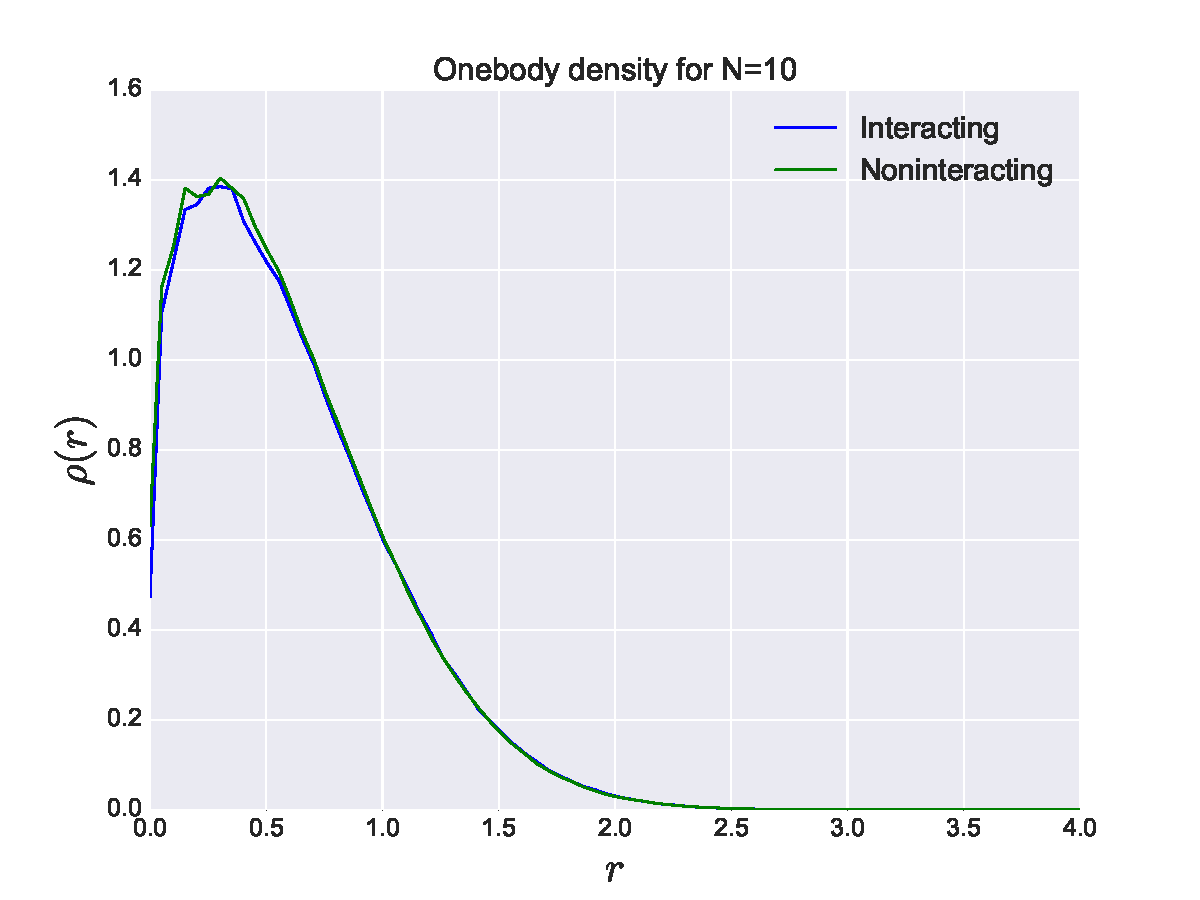
\includegraphics[scale=0.8]{../Results/Onebody_density/onebody.pdf}
			\caption{Radial onebody density for noninteracting ($a=0$) and interacting ($a=0.0043$), using $\omega_z=\omega=\beta=1$, $N=10$ particles in $3$ dimensions, with brute force sampling, running $2^{20}$ Monte Carlo steps.}\label{fig:results_onebody}
		\end{figure}
	\section{Discussion}
	\subsection{The optimal step size}
	\subsubsection{The brute force sampling}\label{sec:Disc_optimal_step_size_brute_force}
	Looking at figure \ref{fig:find_dx_noimportance}, we notice that the error stabilizes quickest for $dx=0.5$ and $dx=1$. Notice that this erorr is \textit{not} estimated using blocking. Therefore, the absolute value of the error is misleading, and we only consider the trend. On a related note, we see that the mean also stabilizes equally quickly in both cases. We therefore choose the $dx$ that gives the highest acceptance ratio, as this minimizes the wasted CPU cycles. This is the case for $dx=0.5$, which explains our choice of step size for the brute-force sampling.
	\subsubsection{Importance sampling}\label{sec:Disc_importance_sampling_step_size}
	The exact same argumentation as in the previous section for figure \ref{fig:find_dx_importance} shows that the error (again \textit{not} corrected for correlations), stabilizes quickest for $dt=0.05$ and $dt=0.1$, and similarly for the mean. Again, we choose the timestep that gives the highest acceptance ratio, which gives $dt=0.05$.
	\subsection{Testing of our code}\label{sec:Desc_testing_code}
	Looking at table \ref{tab:4.1_benchmark_no_Green}, \ref{tab:4.1_benchmark_no_Green_2D} and \ref{tab:4.1_benchmark_no_Green_3D}, we see that the numeric and the analytic energy both reproduce the exact energy, within the uncertainty.  However, the analytic energy runs significantly faster, and has an error of $0$ in the minimum. This justifies using the exact energy for the rest of our simulations.\\
	\linebreak
	The tables showing the benchmarking with importance sampling (table \ref{tab:4.1_benchmark_Green}, \ref{tab:4.1_benchmark_Green_2D} and \ref{tab:4.1_benchmark_Green_3D}) tell a similar story, though the importance sampling is generally somewhat slower for large $N$.\\
	\linebreak
	We also note that the CPU time used by our algorithm suddenly soars when using $N=500$. This is most likely due to the fact that the overhead due to the parallelization at this point becomes insignificant, relative to the time used in the code.
	\subsection{The energy as a function of $\boldsymbol{\alpha}$}\label{sec:Disc_energy_as_a_function_of_alpha}
	We show how the energy varies as a function of $\alpha$ with brute-force sampling in figure \ref{fig:Average_EL_N=100_brute_force} and for importance sampling in figure \ref{fig:Average_EL_N=100_importance}. We note that we manage to hit a minimum at the expected point with both methods, and that this minimum has the correct value in both cases. This suggests that our method is working as expected. We see that importance sampling does not significantly improve the error bound, suggesting that we use sufficiently many steps to attain a stable variance.\\\\
	\linebreak
	 Comparing this with the interacting case, shown for $10$ particles in figure \ref{fig:EL_alpha_N10_interacting}, we see that we get a similar shape - a minimum near $\alpha=0.5$, with a steady increase in energy beyond that point. We also note that the error is relatively small.\\
	 \linebreak
	 We therefore decide to implement brute force sampling in the rest of this project, as it is significantly faster, and does not appear to come at a large cost to accuracy. Whilst it would be possible to use importance sampling with fewer steps, we were unable to get satisfactory results using this method. We therefore use exclusively brute-force sampling for the interacting case.
	 \subsection{Results from the fully interacting system}\label{sec:Disc_Results_from_full}
	 We show how the gradient descent evolves for $N=10$ in the fully interacting system in figure \ref{fig:gradient_descent_interactingN10}. After $40$ iterations, the gradient was less than $10^{-6}$, the convergence was fairly stable, and the optimal $\alpha$ did not change much. We therefore adopt $\alpha = 0.499037$, as stated in table \ref{tab:correct_alpha_interacting} as an acceptable value for $\alpha$.\\
	 \linebreak
	 A similar analysis is done for $N=50$ in figure \ref{fig:gradient_descent_interactingN50}. Also in this case, the gradient descent method gave a small gradient after $40$ iterations (on the order of $10^{-5}$), and the convergence was relatively stable. Furthermore, the optimal $\alpha$ did not change much. We therefore adapt the value $\alpha=0.494033$ quoted in table \ref{tab:correct_alpha_interacting} as our estimate for $\alpha$.\\
	 \linebreak
	 The convergence for $N=100$ was very weak. The gradient stayed above $10^{-3}$ throughout the $40$ iterations, and it varied quite wildly between successive iterations. Furthermore, it was highly sensitive to the starting conditions. Starting with an initial guess of $\alpha=0.3$ gives the $\alpha=0.474419$ shown in table \ref{tab:correct_alpha_interacting}. However, starting with $\alpha=0.49$, gives (after $40$ iterations), $\alpha=0.493261$. Running with this $\alpha$ gives an energy of $E_L=253.0\pm 0.1\ \mathrm{\hbar \omega}$. Similarly, running with the same $\alpha$ as for $N=10$ (i.e. $\alpha=0.499037$) gives a local energy of $E_L=253.12 \pm 0.06\ \mathrm{\hbar \omega}$. These values are slightly lower than for the optimal $\alpha$ found by the gradient descent method. This suggests that the energy is relatively flat close to the minimum. We therefore choose $\alpha=0.493261$ as our correct value of $\alpha$, as this has the lowest energy. Note that this still has a discrepancy of 2.49\% relative to the data found in \cite{Kristiansen2016}.
	 
	 \subsection{The onebody density}\label{sec:Disc_onebody}
	 We show the radial onebody density in figure \ref{fig:results_onebody}. Interpreting this as the probability to find a particle at a certain distance from the origin, shows that the probability is highest a little way out from the origin, and rapidly drops to zero far from the origin. This corresponds to our intuition in the noninteracting system, as we place our bosons a certain distance from the origin initially, and as they do not interact, the spherical potential should lead to a distribution closes to the origin. We also note that the mean of our distribution is at $1.123$, whereas we expected the mean to be at $2/\sqrt{2}\approx 1.128$ (according to appendix \ref{ap:Expectation_value_onebody}). These values are within $0.5\%$ of one another, and are thus in excellent agreement.\\
	 \linebreak
	  We expect the distribution to be shifted slightly to the right in the interacting case, as the bosons no longer have to opportunity to be as closely together. This is not immediately obvious from figure \ref{fig:results_onebody}. We therefore rerun the same algorithm, but let $a=0.1$ (i.e. a much larger repulsive potential). The result of this is shown in figure \ref{fig:disc_onebody}. In this case, the repulsive interaction has a much larger effect, shifting the entire probability distribution outwards. This is in agreement with our intuitive picture of the probability distribution.
	 \begin{figure}[ht!]
	 	\centering
	 	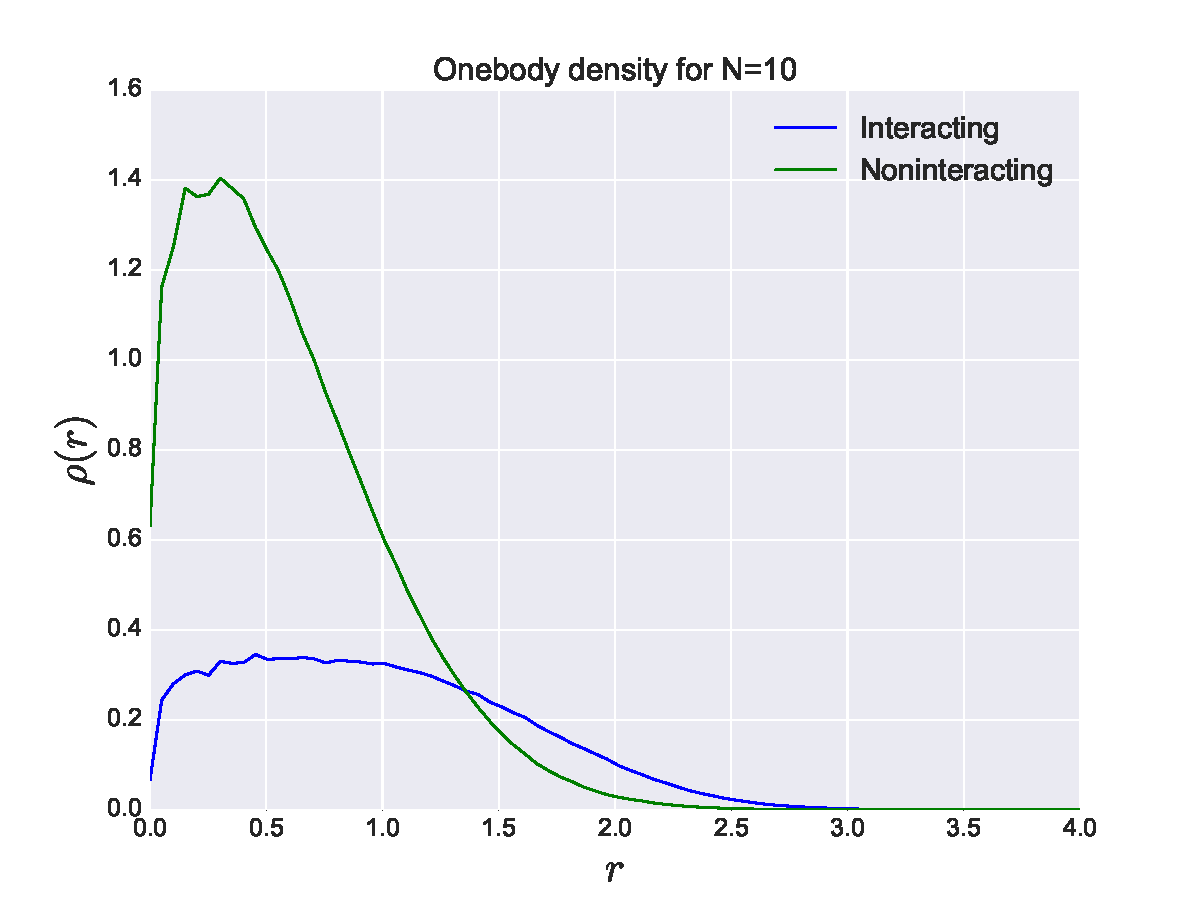
\includegraphics[scale=0.8]{../Results/Onebody_density/onebodyHighAlpha.pdf}
	 	\caption{Same as figure \ref{fig:results_onebody}, but with $a=0.1$.}\label{fig:disc_onebody}
	 \end{figure}
	 \pagebreak
	 \section{Conclusion}
	\subsection{Conclusion}
	We have investigated a system of bosons in a harmonic-oscillator type trap with and without interaction. This investigation is done by using a parallelized variational Monte Carlo code. We choose a class of trial wavefunctions that are in agreement with our physical intuition of the system, and for which we can compute an exact expression for the local energy.\\
	\linebreak
	We find an excellent agreement with analytic results in the noninteracting case, as we are able to reproduce the expected energies, and our variational method gives a minimum energy at the expected value of the variational parameter. We perform a similar analysis in the interacting case. Here, the results are less unequivocal. We are able to attain results that seem reasonable for 10 and 50 bosons, but the results for 100 bosons are somewhat doubtful, as our minimization method was unable to correctly probe the relatively flat energy landscape for $N=100$.  
	
	\subsection{Outlook}
	There is significant future work still to be done. It would be particularly interesting to implement a better minimization method (such as conjugate gradient) to more closely investigate the energy landscape around $\alpha=0.5$ in the interacting system with $100$ particles.\\
	\linebreak
	It would also be very interesting to investigate this system for a larger number of particles, to see how the energy changes. Another extension of these results would be to replace bosons by fermions, to see how the energy changes.\\
	\linebreak
	Finally, an additional point of interest would be to check whether or not the onebody density in the noninteracting case actually corresponds to the exact answer. This answer may be calculated, but we have not done so here, for a lack of time.
	\bibliographystyle{apalike}
	\bibliography{Project1}
	\begin{appendices}
		\section{Analytic expression for the local energy and quantum force}\label{ap:analytic_expression_for_the_local_energy_and_quantum_force}
		\paragraph{First derivative:}
		For particle $k$, $\nabla_k$ is given by:
		\begin{equation}
		\nabla_k\Psi_{T} = \nabla_k\left(\Psi_T(\mathbf{r})=\nabla_k \prod_{i=1}^n\phi(\mathbf{r}_i)\exp\left(\sum_{i<j} u(r_{ij})\right)\right)
		\end{equation}
		Now apply the product rule. For the first term, all terms are unchanged except where $i=k$, giving the first term as:
		\begin{equation}
		\nabla_k \phi(\mathbf{r}_k)\left[ \prod_{i\neq k} \phi(\mathbf{r}_i)\right]\exp\left(\sum_{i<j}u(r_{ij})\right)
		\end{equation}
		The second term is trickier. We can rewrite it as follows:
		\begin{align}
		\prod_{i}\phi(\boldsymbol{r}_{i})\nabla_{k}\left[\exp\left(\sum_{i < j}u(r_{ij})\right)\right]
		= \prod_{i}\phi(\boldsymbol{r}_{i})\nabla_{k}\left[\exp\left(\sum_{j = 1}^{n}\sum_{i = 1}^{j-1}u(r_{ij})\right)\right]
		\label{second term in first derivative}
		\end{align}
		This is calculated by using the chain-rule. To evaluate the innerfunction, we must look
		at \\$1 \le j \le k$, $j = k$ and $j \ge k$. Begining with $1\le  j \le k$,
		the first sum is from $1$ up the kth particle, meaning all terms differentiated before $k$ vanishes
		and we are left with $u(r_{ik})$, thus leaving with us with:
		\begin{align}
		\prod_{i}\phi(\boldsymbol{r}_{i})\nabla_{k}\left[\exp\left(\sum_{j = 1}^{k}\sum_{i = 1}^{k-1}u(r_{ij})\right)\right]
		=
		\prod_{i}\phi(\boldsymbol{r}_{i})\exp{\left(\sum_{i<j}u(r_{ij})\right)}
		\left[\sum_{i = 1}^{k-1}\nabla_{k}u(r_{ik})\right]
		\end{align}
		For $j = k$, we see that the first sum goes from and end up at kth particle, meaning
		this sum vanishes, secondly, the second sum is evaluated at $1 \le i \le k-1$, leaving with
		constants up to $k-1$, thus this term becomes $0$.
		\begin{align}
		\prod_{i}\phi(\boldsymbol{r}_{i})\nabla_{k}\left[\exp\left(\sum_{j = 1}^{n}\sum_{i = 1}^{j-1}u(r_{ij})\right)\right]
		= 0
		\end{align}
		For $j > k$,the first sum goes from $k+1\le j \le n$ and the second $1 \le i \le k$.  The second sum vanishes, because all constants are differentiated away
		except the last term $i = k$. This leaves us with:
		\begin{align}
		\prod_{i}\phi(\boldsymbol{r}_{i})\nabla_{k}\left[\exp\left(\sum_{j = k+1}^{n}\sum_{i = 1}^{k}u(r_{ij})\right)\right]
		= \prod_{i}\phi(\boldsymbol{r}_{i})
		\exp{\left(\sum_{i<j}u(r_{ij})\right)}
		\left[\sum_{j = k + 1}^{n}\nabla_{k}u(r_{kj})\right]
		\end{align}
		We can now write the second term as \ref{second term in first derivative}):
		\begin{align}\label{combined sum}
		\prod_{i}\phi(\boldsymbol{r}_{i})
		\exp{\left(\sum_{i<j}u(r_{ij})\right)}
		\left[\sum_{j = k + 1}^{n}\nabla_{k}u(r_{kj}) +
		\left[\sum_{i = 1}^{k-1}\nabla_{k}u(r_{ik})\right]\right]
		\end{align}
		%CHECK THIS EQUATION
		This can be rewritten to:
		\begin{align}
		\prod_{i}\phi(\boldsymbol{r}_{i})
		\exp{\left(\sum_{i<j}u(r_{ij})\right)}
		\left[\sum_{j \neq k}\nabla_{k}u(r_{kj})\right]
		\end{align}
		Thus the first derivative of the trial wavefunction
		can be written as:
		\begin{align}
		\nabla_{k}\Psi_{T} =
		\nabla_k \phi(\mathbf{r}_k)\left[ \prod_{i\neq k} \phi(\mathbf{r}_i)\right]\exp\left(\sum_{i<j}u(r_{ij})\right)
		+ \prod_{i}\phi(\boldsymbol{r}_{i})
		\exp{\left(\sum_{i<j}u(r_{ij})\right)}
		\left[\sum_{j \neq k}u(r_{kj})\right]
		\end{align}
		\paragraph{Second derivative:}
		Lastly we will calculate the second derivative of the trial function, where we
		use the product rule and the chain rule. We will then obtain the following:
		\begin{align*}
		\begin{split}
		\nabla_{k}^2\Psi_{T} =
		\underbrace{\nabla_k^2 \phi(\mathbf{r}_k)\left[ \prod_{i\neq k} \phi(\mathbf{r}_i)\right]\exp\left(\sum_{i<j}u(r_{ij})\right)}_{\mathrm{I}} +\\
		\underbrace{2\left(\nabla_k \phi(\mathbf{r}_k)\left[ \prod_{i\neq k} \phi(\mathbf{r}_i)\right]
			\exp{\left(\sum_{i<j}u(r_{ij})\right)}
			\left[\sum_{j \neq k}\nabla_{k}u(r_{kj})\right]\right)}_{\mathrm{II}} +
		\\
		\underbrace{\prod_{i}\phi(\boldsymbol{r}_{i})
			\exp{\left(\sum_{i<j}u(r_{ij})\right)}
			\left[\sum_{j \neq k}\nabla_{k}u(r_{kj})\right]^2}_{\mathrm{III}} +
		\\
		\underbrace{\prod_{i}\phi(\boldsymbol{r}_{i})
			\exp{\left(\sum_{i<j}u(r_{ij})\right)}
			\left[\sum_{j \neq k}\nabla_{k}\nabla_{k}u(r_{kj})\right]}_{\mathrm{IV}}
		\end{split}
		\end{align*}
		Where the derivatives of the different parts are obtained from previous.
		We will now divide the second derivative by the trial wavefunction, and obtain:
		\begin{align}
		\frac{1}{\Psi_{T}}\nabla_{k}^2\Psi_{T} =
		\underbrace{\frac{\nabla_{k}^2\phi{(\boldsymbol{r}_{k})}}{\phi(\boldsymbol{r}_{\phi(\boldsymbol{r}_{k})})}}_{\mathrm{I}}
		+ \underbrace{2\frac{\nabla_{k}\phi(\boldsymbol{r}_{k})}{\phi{(\boldsymbol{r}_{k})}}\sum_{j\neq k}\nabla_{k}u(r_{kj})}_{\mathrm{II}}
		+ \underbrace{\left(\sum_{j\neq k}\nabla_{k} u(r_{kj})\right)^2}_{\mathrm{III}} +
		\underbrace{\left[\sum_{j \neq k}\nabla_{k}\nabla_{k}u(r_{kj})\right]}_{\mathrm{IV}}
		\end{align}
		We will now carry out the differentiation in term (II), (III) and (IV). Begining with the
		(II), by using the chain rule we can rewrite (II) as:
		\begin{align*}
		2\frac{\nabla_{k}\phi(\boldsymbol{r}_{k})}{\phi{(\boldsymbol{r}_{k})}}\sum_{j\neq k}\pdv{u(r_{kj})}{r_{kj}}\pdv{r_{kj}}{\boldsymbol{r}_{k}} =
		2\frac{\nabla_{k}\phi(\boldsymbol{r}_{k})}{\phi{(\boldsymbol{r}_{k})}}\left(\sum_{j\neq k}\frac{\boldsymbol{r}_{k} - \boldsymbol{r}_{j}}{r_{kj}}u'(r_{kj})\right)
		\end{align*}
		Where we have used $\nabla_{k} r_{kj} = (\boldsymbol{r}_{k} - \boldsymbol{r}_{j})/r_{kj}$.
		Looking at (III), we can write out the square into two factors. The second paranthese the summation index is replaced by a
		dummy index $i$. Thus will look as:
		\begin{align}
		\left(\sum_{j\neq k}\nabla_{k} u(r_{kj})\right)^2 = \left(\sum_{j\neq k}\nabla_{k} u(r_{kj})\right)\left(\sum_{i\neq k}\nabla_{k} u(r_{ki})\right)
		\end{align}
		From (II) we found the derivative of this function. Thus this can be expressed as (combining also the double sum):
		\begin{align}
		\left(\sum_{j\neq k}\nabla_{k} u(r_{kj})\right)^2 =
		\sum_{i, j\neq k}\left(\frac{\boldsymbol{r}_{k} - \boldsymbol{r}_{j}}{r_{kj}}\right)
		\left(\frac{\boldsymbol{r}_{k} - \boldsymbol{r}_{i}}{r_{ki}}\right)u'(r_{kj})u'(r_{ki})
		\end{align}
		The last part (IV), we must use the chain rule and product rule together. We will obtain
		the following term:
		\begin{align}
		\sum_{j \neq k}\nabla_{k}\nabla_{k}u(r_{kj}) =
		\sum_{j \neq k}\nabla_{k}\left(
		\left(\frac{\boldsymbol{r}_{k} - \boldsymbol{r}_{j}}{r_{kj}}\right)^2 u''(r_{kj}) + u'(r_{kj})\nabla_{k}
		\left(\frac{\boldsymbol{r}_{k} - \boldsymbol{r}_{j}}{r_{kj}}\right)\right)
		\end{align}
		Note that this is a unit vector squared:
		\begin{align}
		\left(\frac{\boldsymbol{r}_{k} - \boldsymbol{r}_{j}}{r_{kj}}\right)^2 = 1
		\end{align}
		and the last part is found by using the qoutient rule. This is the divergence to the vectors, since we are evaluating for
		specific particle k, and gradient to scalar (we must look for all combination of k particle):
		\begin{align}
		\nabla_{k}
		\left(\frac{\boldsymbol{r}_{k} - \boldsymbol{r}_{j}}{r_{kj}}\right)
		= \frac{r_{kj}\left(\nabla_{k}\cdot\boldsymbol{r}_{k}-
			\nabla_{k}\cdot\boldsymbol{r}_{j}\right) -
			(\boldsymbol{r}_{k}-\boldsymbol{r}_{j})\nabla_{k}r_{kj}}{r_{kj}^2}
		\end{align}
		This simply becomes:
		\begin{align}
		\nabla_{k}
		\left(\frac{\boldsymbol{r}_{k} - \boldsymbol{r}_{j}}{r_{kj}}\right)
		= \frac{3r_{kj}^2 - \boldsymbol{r}^2_{k} + 2(\boldsymbol{r}_{k}\cdot \boldsymbol{r}_{j}) - \boldsymbol{r}^2_{j}}{r_{kj}^3}
		\end{align}
		Note that $r_{kj} - \boldsymbol{r}^2_{k} + 2(\boldsymbol{r}_{k}\cdot \boldsymbol{r}_{j}) - \boldsymbol{r}^2_{j} = 0$, this leaves us with:
		\begin{align}
		\nabla_{k}
		\left(\frac{\boldsymbol{r}_{k} - \boldsymbol{r}_{j}}{r_{kj}}\right)
		= \frac{2}{r_{kj}}
		\end{align}
		Thus expression (IV) can be expressed as:
		\begin{align}
		\sum_{j \neq k}\nabla_{k}\nabla_{k}u(r_{kj}) =
		\sum_{j \neq k}\nabla_{k}\left(u''(r_{kj}) + \frac{2}{r_{kj}}u'(r_{kj})
		\right)
		\end{align}
		Combining (I), (II), (III) and (IV), we we will get that the second derivative
		of the trial function is:
		\begin{align}
		\begin{split}
		\frac{1}{\Psi_{T}}\nabla_{k}^2\Psi_{T} =
		\frac{\nabla_{k}^2\phi{(\boldsymbol{r}_{k})}}{\phi(\boldsymbol{r}_{k})}
		+
		2\frac{\nabla_{k}\phi(\boldsymbol{r}_{k})}{\phi{(\boldsymbol{r}_{k})}}\left(\sum_{j\neq k}\frac{\boldsymbol{r}_{k} - \boldsymbol{r}_{j}}{r_{kj}}u'(r_{kj})\right)
		+\\
		\sum_{i, j\neq k}\left(\frac{\boldsymbol{r}_{k} - \boldsymbol{r}_{j}}{r_{kj}}\right)
		\left(\frac{\boldsymbol{r}_{k} - \boldsymbol{r}_{i}}{r_{ki}}\right)u'(r_{kj})u'(r_{ki})
		+
		\sum_{j \neq k}\left(u''(r_{kj}) + \frac{2}{r_{kj}}u'(r_{kj})\right)
		\end{split}
		\end{align}
		\paragraph{Local energy:} Now that we have the second derivative of the
		trial-function, we can write out the analytical expression for the local energy.
		Recall that:
		\begin{align}
		E_{L}(\boldsymbol{r}) = \frac{1}{\Psi_{T}}H\Psi_{T} =
		\frac{1}{\Psi_{T}}\left[\sum_{i}^{N}\left(-\frac{\hbar^{2}}{2m}\nabla^{2}_{i}
		+ V_{ext}(\boldsymbol{r}_{i})\right) + \sum_{i < j}^{N}V_{int}(
		\boldsymbol{r}_{i},\boldsymbol{r}_{j})\right]\psi_{T}
		\end{align}
		The second derivative written explicitly is:
		\begin{align}
		\begin{split}
		\frac{1}{\Psi_{T}}\nabla^{2}_{k}\Psi_{T} = 4\alpha\boldsymbol{Q}_{k}^{2} - 4\alpha\boldsymbol{Q}_{k}
		\sum_{j\neq k}\left(\frac{\boldsymbol{r}_{k} - \boldsymbol{r}_{j}}{r_{kj}}u'(r_{kj})\right)
		+\\
		\sum_{i,j\neq k}\frac{\boldsymbol{r}_{k}\cdot\boldsymbol{r}_{k} - \boldsymbol{r}_{k}\cdot\boldsymbol{r}_{j} - \boldsymbol{r}_{k}\cdot\boldsymbol{r}_{i} + \boldsymbol{r}_{i}\cdot\boldsymbol{r}_{j}}{r_{kj}r_{ki}}u'(r_{ki})u'(r_{kj})
		\\
		+ \sum_{j \neq k}\left(u''(r_{kj}) + \frac{2}{r_{kj}}u'(r_{kj})\right)
		\end{split}
		\end{align}
		Where $\boldsymbol{Q}_{k} = \left(x_{k}\hat{i} + y_{k}\hat{j} + \beta z_{k}\hat{k}\right)$,
		and the first and second derivative of $u(r_{kj})$ is:
		\begin{align}
		u'(r_{kj}) =
		\begin{cases}
		\infty &, r_{kj} \le a\\
		\frac{a}{r_{kj}^{2} - ar_{kj}} &, r_{kj} > a
		\end{cases}
		\label{udiv}
		\end{align}
		and
		\begin{align}
		u''(r_{kj}) =
		\begin{cases}
		\infty &, r_{kj} \le a\\
		\frac{a^{2} - 2ar_{kj}}{\left(r_{kj}^{2} - ar_{kj}\right)^{2}} &, r_{kj} > a
		\end{cases}
		\label{udivdiv}
		\end{align}
		Thus the analytical local energy for a group of particle is:
		\begin{align}
		\begin{split}
		E_{L} = -\frac{\hbar^{2}}{2m}\sum_{k}\left[
		4\alpha^{2}\boldsymbol{Q}_{k}^{2} - 4\alpha\boldsymbol{Q}_{k} + \sum_{j \neq k}\left(\frac{\boldsymbol{r}_{k} - \boldsymbol{r}_{j}}{r_{kj}}u'(r_{kj})\right)\right.
		\\ \left. + \sum_{i,j \neq k}\left(\frac{\boldsymbol{r}\cdot\boldsymbol{r} + \boldsymbol{r}_{j}\cdot\boldsymbol{r}_{i} - \boldsymbol{r}_{j}\cdot\boldsymbol{r}_{k} -\boldsymbol{r}_{k}\cdot\boldsymbol{r}_{i}}{r_{ki}r_{kj}}u'(r_{ki})u'(r_{kj})\right)\right.
		\\
		\left. + \sum_{j \neq k}\left(u''(r_{kj} + \frac{2}{r_{kj}}u'(r_{kj}))\right)\right]
		+ \sum_{k}V_{ext}(\boldsymbol{r}_{k}) + \sum_{i < j}V_{int}(\boldsymbol{r}_{i}, \boldsymbol{r}_{j})
		\end{split}
		\end{align}
		This expression includes the situation where particles interact with each other.
		Now if we assume the particles does not interact with each other, we then have:
		\begin{align}
		E_{L} = \sum_{k}\left(4\alpha^{2}\boldsymbol{Q}_{k} + V_{ext}(\boldsymbol{r}_{k}) \right)
		\end{align}
		\paragraph{Quantum force/Drift force:}
		The quantum/drift force is defined to be:
		\begin{align}
		\boldsymbol{F}_{i} = 2\frac{\nabla\Psi_{T}}{\Psi_{T}}
		\end{align}
		Using the first derivative we just derived above this expression will look like:
		\begin{align}
		\boldsymbol{F}_{i} = 2\frac{\nabla_k \phi(\boldsymbol{r}_{k})}{\phi(\boldsymbol{r}_{k})}
		+
		2\sum_{j \neq k}\frac{\boldsymbol{r}_{k} - \boldsymbol{r}_{j}}{r_{kj}}u'(r_{kj})
		= -4\alpha\boldsymbol{Q}_{i} +
		2\sum_{j \neq k}\frac{\boldsymbol{r}_{k} - \boldsymbol{r}_{j}}{r_{kj}}u'(r_{kj})
		\end{align}
		Where $\boldsymbol{Q}_{i} = x_{i}\hat{i} + y_{i}\hat{j} + \beta z_{i}\hat{k}$ and
		$u'(r_{kj})$ is given in (\ref{udiv}). This is for a interacting case, since
		the distance between two particle and the gradient $kj$'th particle appears.
		Further notice that the quantum force can be written
		as $3\cross N$ matrix, where $N$ is number of particles in the system.
		For a non-interacting case, we have:
		\begin{align}
		\boldsymbol{F}_{i} = -4\alpha\boldsymbol{Q}_{i}
		\end{align}
		\section{Finding the derivative of the local energy}\label{ap:derivative_of_local_energy}
		The local energy, $E_L$ is given by:
		\begin{equation}
		E_L=\langle \Psi_T | H| \Psi_T \rangle
		\end{equation}
		We now want to find the derivative of the expectation value of the local energy $\langle E_{L}\rangle$
		with respect to the variational parameter $\alpha$. Before we do that we must normalize the wavefunction:
		\begin{align}
		\ket{\Psi_{T}} = \frac{\ket{\Psi_{T}}}{\sqrt{\braket{\Psi_{T}}}}
		\end{align}
		The expectation value of the local energy is then:
		\begin{align}
		\langle E_{L} \rangle = \frac{\bra{\Psi_{T}}E_{L}\ket{\Psi_{T}}}{\braket{\Psi_{T}}}
		\end{align}
		Notice that can be written as:
		\begin{align}
		\langle E_{L} \rangle = \frac{\bra{\Psi_{T}}E_{L}\ket{\Psi_{T}}}{\braket{\Psi_{T}}}
		= \frac{1}{\braket{\Psi_{T}}}\int..\int \Psi_{T}^{*}E_{L}\Psi_{T}\dd{\bold{r}_{1}}..\dd{\bold{r}_{N}}
		\end{align}
		Using the definition of $E_{L}$ and we know that the wavefunction is real, we get that:
		\begin{align}
		\langle E_{L} \rangle = \frac{1}{\braket{\Psi_{T}}}\int..\int \Psi_{T}^{*}\left(\frac{1}{\Psi_{T}}H\Psi_{T}\right)\Psi_{T}\dd{\bold{r}_{1}}..\dd{\bold{r}_{N}}
		= \frac{1}{\braket{\Psi_{T}}}\int..\int H\Psi_{T}\Psi_{T}\dd{\bold{r}_{1}}..\dd{\bold{r}_{N}}
		\end{align}
		Thus this can be written as:
		\begin{align}
		\langle E_{L} \rangle = \frac{\bra{\Psi_{T}}H\ket{\Psi_{T}}}{\braket{\Psi_{T}}}
		\end{align}
		By using the product rule and differentiating this with respect to $\alpha$,
		we will get:
		\begin{align}
		\pdv{\langle E_{L} \rangle }{\alpha} = \frac{1}{\braket{\Psi_{T}}}\pdv{\bra{\Psi_{T}}H\ket{\Psi_{T}}}{\alpha}
		+ \bra{\Psi_{T}}H\ket{\Psi_{T}}\pdv{\alpha}\left(\frac{1}{\braket{\Psi_{T}}}\right)
		\label{proddiff}
		\end{align}
		The first expression is:
		\begin{align}
		\frac{1}{\braket{\Psi_{T}}}\pdv{\bra{\Psi_{T}}H\ket{\Psi_{T}}}{\alpha}
		=
		\frac{1}{\braket{\Psi_{T}}}\pdv{\alpha}\int..\int\Psi_{T}^{*}H\Psi_{T}\dd{\bold{r}_{1}}..\dd{\bold{r}_{N}}
		\end{align}
		Taking the derivative into the integral and apply the product rule, we will obtain:
		\begin{align}
		\frac{1}{\braket{\Psi_{T}}}\int..\int\pdv{\Psi_{T}^{*}}{\alpha}H\Psi_{T}
		+   \Psi_{T}^{*}\pdv{H}{\alpha}\Psi_{T}
		+   \Psi_{T}^{*}H\pdv{\Psi_{T}}{\alpha}\dd{\bold{r}_{1}}..\dd{\bold{r}_{N}}
		\end{align}
		Since the hamiltonian does not depend on $\alpha$ we have:
		\begin{align}
		\frac{1}{\braket{\Psi_{T}}}\int..\int\underbrace{\pdv{\Psi_{T}^{*}}{\alpha}H\Psi_{T}}_{I}
		+   \underbrace{\Psi_{T}^{*}H\pdv{\Psi_{T}}{\alpha}}_{II}\dd{\bold{r}_{1}}..\dd{\bold{r}_{N}}
		\end{align}
		We now wish to include the local energy in the integral, to do this we must
		do some algebra. Consider the first expression ($I$):
		\begin{align}
		\frac{1}{\braket{\Psi_{T}}}\int..\int \pdv{\Psi_{T}^{*}}{\alpha}H\Psi_{T}\dd{\bold{r}_{1}}..\dd{\bold{r}_{N}}
		\end{align}
		By dividing and multiplying with $\Psi_{T}^{*}$ and $\Psi_{T}$ on the left and right for the
		hamiltonian operator, we can write $I$ as:
		\begin{align}
		\begin{split}
		\frac{1}{\braket{\Psi_{T}}}\int..\int \frac{\Psi_{T}^{*}}{\Psi_{T}^{*}}\pdv{\Psi_{T}^{*}}{\alpha}H\Psi_{T}\frac{\Psi_{T}}{\Psi_{T}}\dd{\bold{r}_{1}}..\dd{\bold{r}_{N}}
		=
		\\
		\frac{1}{\braket{\Psi_{T}}}\int..\int \frac{|\Psi_{T}|^{2}}{\Psi_{T}}\pdv{\Psi_{T}^{*}}{\alpha}E_{L}\dd{\bold{r}_{1}}..\dd{\bold{r}_{N}}
		\\
		= \langle \frac{E_{L}}{\Psi_{T}}\pdv{\Psi_{T}}{\alpha}\rangle
		\label{result1}
		\end{split}
		\end{align}
		Expression (II) is more trickier to handle, since we know that the hamiltionian
		operator is hermitian and the wavefunction is real, we know that:
		\begin{align}
		\bra{a}H\ket{b}^{*} = \bra{b}H\ket{a}
		\end{align}
		We will now write expression (I) and (II) in Dirac notation. Expression (I) will
		look like:
		\begin{align}
		\frac{1}{\braket{\Psi_{T}}}\int..\int \frac{\Psi_{T}^{*}}{\Psi_{T}^{*}}\pdv{\Psi_{T}^{*}}{\alpha}H\Psi_{T}\dd{\bold{r}_{1}}..\dd{\bold{r}_{N}}
		= \bra{\Psi_{T}}\frac{1}{\Psi_{T}}\pdv{\Psi_{T}}{\alpha}H\ket{\Psi_{T}}
		\label{dirac1}
		\end{align}
		Expression (II) will look like:
		\begin{align}
		\frac{1}{\braket{\Psi_{T}}}\int..\int\Psi_{T}^{*}H\pdv{\Psi_{T}}{\alpha}\frac{\Psi_{T}}{\Psi_{T}}\dd{\bold{r}_{1}}..\dd{\bold{r}_{N}}
		= \bra{\Psi_{T}}H\pdv{\Psi_{T}}{\alpha}\frac{1}{\Psi_{T}}\ket{\Psi_{T}}
		\label{dirac2}
		\end{align}
		Notice that (\ref{dirac1}) and (\ref{dirac2}) are just the conjugate of each oher, thus:
		\begin{align}
		\bra{\Psi_{T}}H\pdv{\Psi_{T}}{\alpha}\frac{1}{\Psi_{T}}\ket{\Psi_{T}}^{*}
		=
		\bra{\Psi_{T}}\frac{1}{\Psi_{T}}\pdv{\Psi_{T}}{\alpha}H\ket{\Psi_{T}}
		\end{align}
		Since (\ref{dirac1}) is equal to (\ref{result1}) then (\ref{dirac1}) must also equal the result from
		(\ref{result1}). Thus:
		\begin{align}
		\frac{1}{\braket{\Psi_{T}}}\int..\int\pdv{\Psi_{T}^{*}}{\alpha}H\Psi_{T}
		+   \Psi_{T}^{*}H\pdv{\Psi_{T}}{\alpha}\dd{\bold{r}_{1}}..\dd{\bold{r}_{N}}
		= 2 \langle \frac{E_{L}}{\Psi_{T}}\pdv{\Psi_{T}}{\alpha} \rangle
		\end{align}
		Now differentiating the second expression in (\ref{proddiff}):
		\begin{align}
		\bra{\Psi_{T}}H\ket{\Psi_{T}}\pdv{\alpha}\left(\frac{1}{\braket{\Psi_{T}}}\right)
		= -\frac{\bra{\Psi_{T}}H\ket{\Psi_{T}}}{\braket{\Psi_{T}}^{2}}\pdv{\braket{\Psi_{T}}}{\alpha}
		\end{align}
		Writing the last expression as an integral:
		\begin{align}
		-\frac{\bra{\Psi_{T}}H\ket{\Psi_{T}}}{\braket{\Psi_{T}}^{2}}\pdv{\braket{\Psi_{T}}}{\alpha}
		= -\frac{\bra{\Psi_{T}}H\ket{\Psi_{T}}}{\braket{\Psi_{T}}^{2}}\int..\int \pdv{\Psi_{T}^{*}}{\alpha}\Psi_{T} +
		\Psi_{T}^{*}\pdv{\Psi_{T}}{\alpha}\dd{\bold{r}_{1}}..\dd{\bold{r}_{N}}
		\end{align}
		we clearly see that:
		\begin{align}
		-\frac{\bra{\Psi_{T}}H\ket{\Psi_{T}}}{\braket{\Psi_{T}}^{2}}\int..\int \pdv{\Psi_{T}^{*}}{\alpha}\Psi_{T}
		+
		\Psi_{T}^{*}\pdv{\Psi_{T}}{\alpha}\dd{\bold{r}_{1}}..\dd{\bold{r}_{N}}
		=
		-2\frac{\bra{\Psi_{T}}H\ket{\Psi_{T}}}{\braket{\Psi_{T}}^{2}}\int..\int \pdv{\Psi_{T}^{*}}{\alpha}\Psi_{T}\dd{\bold{r}_{1}}..\dd{\bold{r}_{N}}
		\end{align}
		We will now divide with $\frac{\Psi_{T}^{*}}{\Psi_{T}^{*}}$,
		use the definition of the expectation value of the local energy and derivative of the wavefunction with respect to $\alpha$,
		This can also be written as:
		\begin{align}
		-2\frac{\bra{\Psi_{T}}H\ket{\Psi_{T}}}{\braket{\Psi_{T}}^{2}}\int..\int \Psi_{T}^{*}\Psi_{T}\left(\frac{1}{\Psi_{T}}\pdv{\Psi_{T}^{*}}{\alpha}\right)\dd{\bold{r}_{1}}..\dd{\bold{r}_{N}}
		= -2\langle E_{L} \rangle \langle \frac{1}{\Psi_{T}}\pdv{\Psi}{\alpha}\rangle
		\end{align}
		thus:
		\begin{align}
		\bra{\Psi_{T}}H\ket{\Psi_{T}}\pdv{\alpha}\left(\frac{1}{\braket{\Psi_{T}}}\right)
		= -2\langle E_{L} \rangle \langle \frac{1}{\Psi_{T}}\pdv{\Psi}{\alpha}\rangle
		\end{align}
		Combining the first and second expression the derivative of the local energy can
		be expressed as:
		\begin{align}
		\pdv{\langle E_{L} \rangle }{\alpha} =
		2\left(\langle \frac{E_{L}}{\Psi_{T}}\pdv{\Psi_{T}}{\alpha} \rangle -
		\langle E_{L} \rangle \langle \frac{1}{\Psi_{T}}\pdv{\Psi}{\alpha}\rangle\right)
		\end{align}
		\section{The dimensionless Hamiltonian}\label{ap:dimensionless_hamiltonian}
		We aim to demonstrate that the Hamiltonian in equation \ref{eq:general_Hamiltonian} is equivalent to the Hamiltonian shown in equation \ref{eq:Hamiltonian_dimensionless} under the coordinate transformation:
		\begin{equation}
		\boldsymbol{r}\rightarrow \frac{\boldsymbol{r}}{a_{ho}}=\boldsymbol{r} \sqrt{\frac{m\omega}{\hbar}} \quad E\rightarrow \frac{E}{\hbar \omega}
		\end{equation}
		Where $a_{ho}=(h/m\omega)^{1/2}$. To show this, note first that the gradient operator under this transformation transforms as:
		\begin{equation}
		\nabla \rightarrow \sqrt{\frac{\hbar}{m\omega}} \nabla
		\end{equation}
		We now introduce this coordinate transformation into our Hamiltonian. This gives:
		\begin{equation}
		H\rightarrow H=\sum_{i=1}^{N}\left(-\frac{\hbar^2}{2m}\frac{\omega m}{\hbar}\nabla_i^2+\frac{1}{2}m\omega^2 \frac{\hbar}{m\omega}(x_i^2+y_i^2 +\omega_z^2 z_i^2) \right)+\sum_{i<j}^N V_{int}(\boldsymbol{r}_i, \boldsymbol{r}_j)
		\end{equation}
		Which can be rewritten as:
		\begin{equation}
		H=\frac{\hbar \omega}{2}\sum_{i=1}^N\left(-\nabla^2 +\frac{\hbar \omega}{2}\left(x_i^2+y_i^2 + \frac{\omega_z^2}{\omega^2}z_i^2\right)\right)+\sum_{i<j}^N V_{int}(\boldsymbol{r}_i, \boldsymbol{r}_j)
		\end{equation}
		Relabeling the energy and defining $\gamma=\omega_z/\omega$ gives:
		\begin{equation}
		H=\frac{1}{2}\sum_{i=1}^N \left(-\nabla_i^2 +x_i^2+y_i^2+\gamma z_i^2\right)+\sum_{i<j}^N V_{int}(\boldsymbol{r}_i, \boldsymbol{r}_j)
		\end{equation}
		Which is exactly equation \ref{eq:Hamiltonian_dimensionless}.
		
		\section{Deriving an approximate expression for the onebody density}\label{ap:approximte_onebody_density}
		We require that the spatial integral over the onebody density, $\rho(\boldsymbol{r_1})$ equals the total number of particles $N$. As we are only interested in the radial component of the onebody density, we consider only $\rho(r)$. This requirement can then be written as:
		\begin{equation}
		N=\int d^3 \boldsymbol{r} \rho(r)
		\end{equation} 
		Which gives, in spherical coordinates:
		\begin{equation}
		N=4\pi \int_0^{\infty}dr\  r^2 \rho(r)
		\end{equation}
		We now discretize this integral radius, choosing to integrate from $0$ to $r_{\mathrm{max}}$, where we choose $r_{\mathrm{max}}$ larger than the largest distance any particle deviates from the origin. This interval is divided into $M$ points, with a spacing of $\Delta r$. The discretized version of the integral then becomes:
		\begin{equation}
		N\approx 4\pi \sum_{i=1}^M r_i^2 \rho(r_i) \Delta r
		\end{equation}
		From which it follows that the onebody density can be computed as:
		\begin{equation}
		\rho(r_i)\approx \frac{N_i}{4\pi r_i^2 \Delta r}
		\end{equation}
		Where $N_i$ is the number of particles in the spherical shell with radius $r_i$ to $r_i+\Delta r$.
		\section{Finding the expectation value of the onebody density}\label{ap:Expectation_value_onebody}
		If we choose to interpret the onebody density as the probability of finding a single particle at a distance $r$ from the origin, then we can compute the expected distance from the origin for the isotropic harmonic oscillator. The exact wavefunction (in atomic units) is (according to \cite{Griffiths2004}) given by:
		\begin{equation}
		\psi(r)=A\exp\left(-\frac{r^2}{2}\right)
		\end{equation}
		Where $A$ is a normalization factor. We compute this as:
		\begin{equation}
		1=\langle \psi | \psi \rangle = |A|^2 \int_0^{2\pi}\int_0^{\pi} \int_0^{\infty} d\phi d\theta dr\ r^2 \sin \theta \exp \left(-r^2\right) = 4\pi |A|^2\int_0^{\infty}dr\ r^2\exp(-r^2)
		\end{equation}
		Looking up the integral gives:
		\begin{equation}
		1= |A|^2 \pi^{3/2}
		\end{equation}
		Choosing a positive real value gives the normalization factor as:
		\begin{equation}
		A=\pi^{-3/2}
		\end{equation}
		The expected value of the distance from the origin is now given by:
		\begin{equation}
		\langle r \rangle =\pi^{-3/2}\int_0^{2\pi}\int_0^{\pi} \int_0^{\infty}d\phi d\theta dr\ r^3\sin \theta \exp (-r^2)=\frac{2}{\sqrt{\pi}}\approx 1.128
		\end{equation}
	\end{appendices}
\end{document}